% !TeX spellcheck = en_GB
\section{Atmospheric River map}
\label{sec:atm_riv}
%%% Atmospheric river maps %%%%%%%%%%%%%%%%%%%%%%%%%%%%%%%%%%%%%
% !TeX spellcheck = en_GB
\begin{figure}[h!]
	\centering
	%%%%%% 20/12
	\begin{subfigure}[b]{0.49\textwidth}
		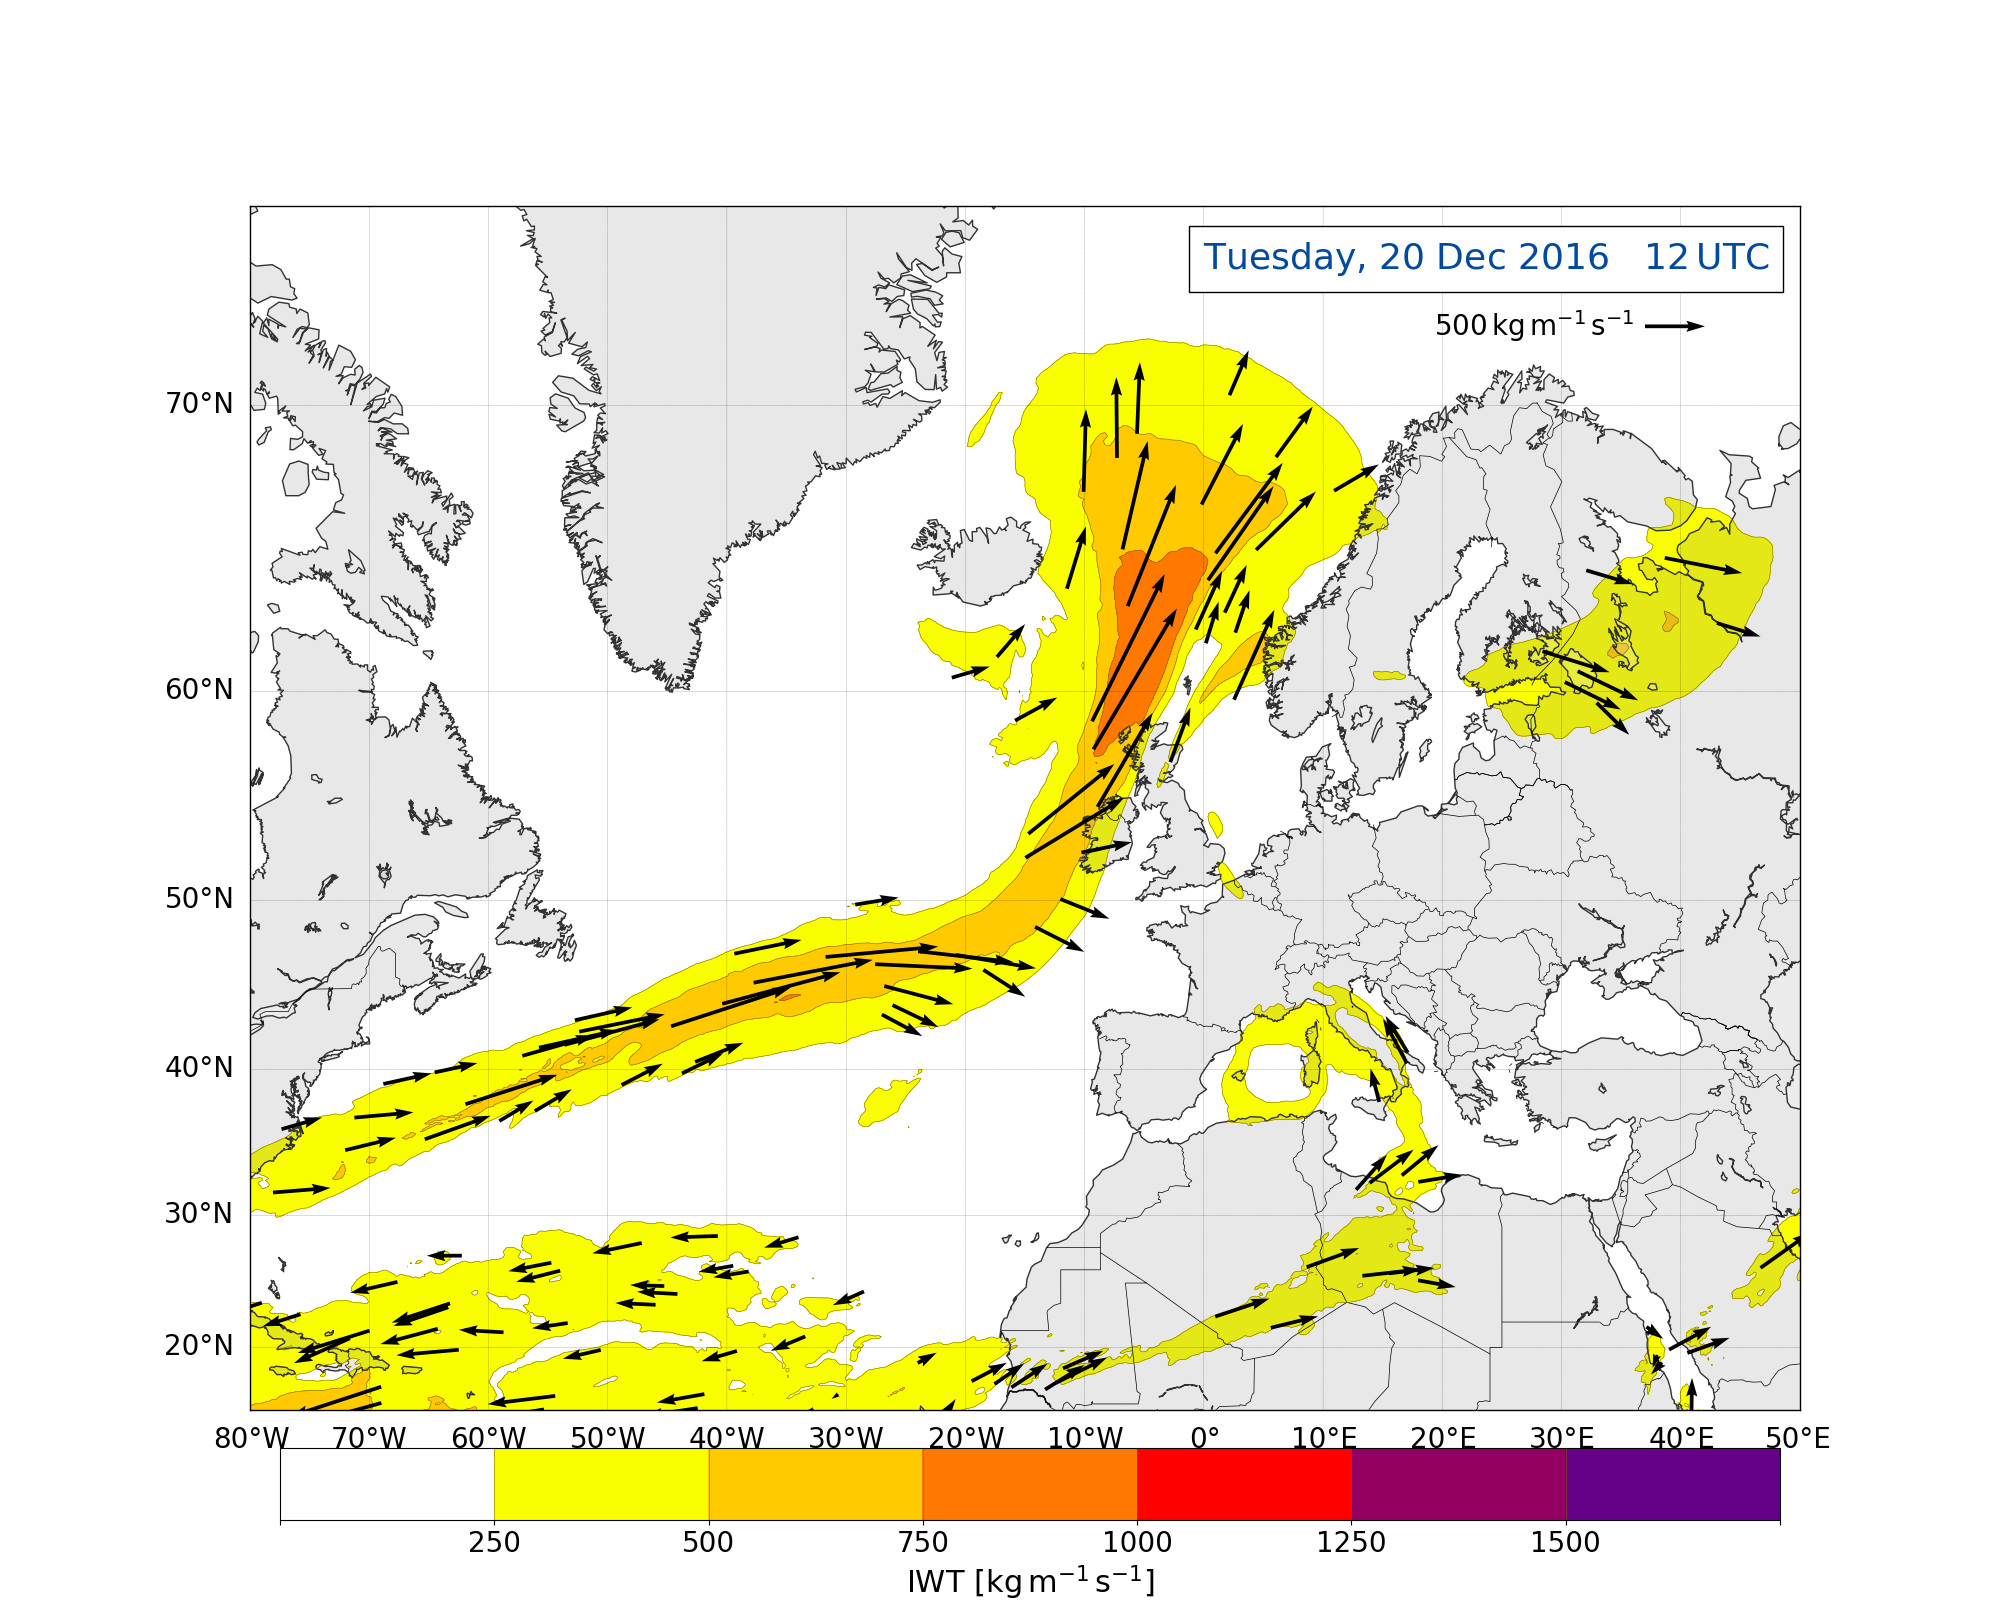
\includegraphics[trim={4.2cm 3.9cm 4.3cm 5.1cm},clip,
		width=\textwidth]{./fig_Atm_Riv/20161220_12}
		\caption{}\label{fig:AR20}
	\end{subfigure}
	%%%%%% 21/12
	\begin{subfigure}[b]{0.49\textwidth}
		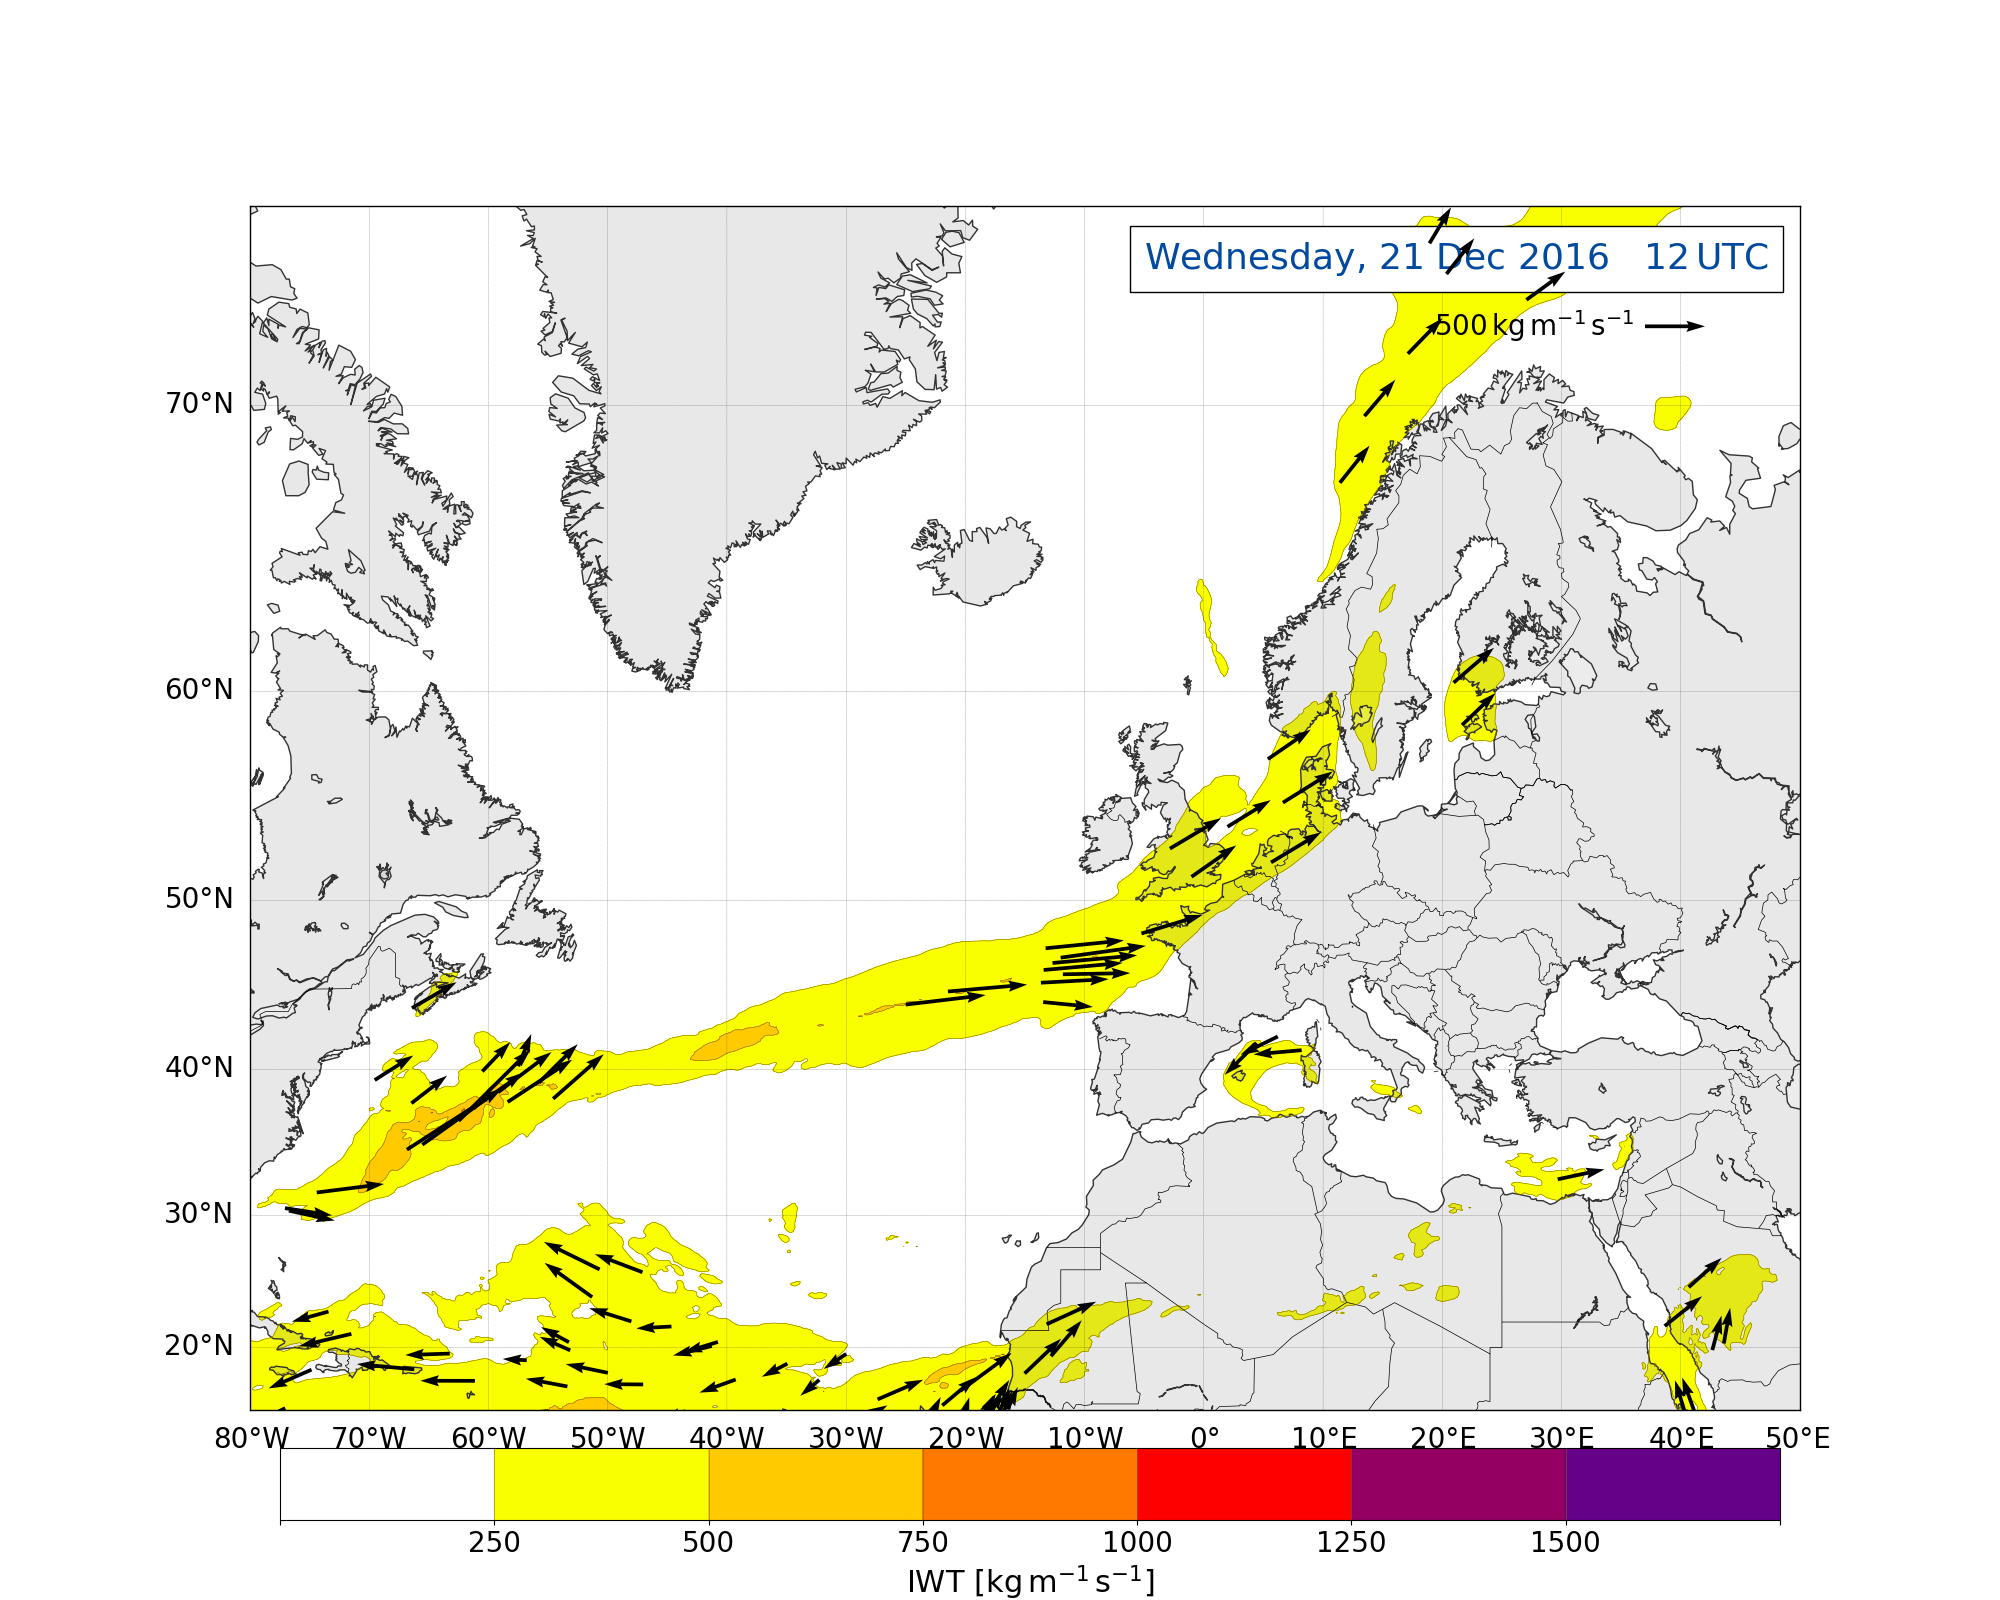
\includegraphics[trim={4.2cm 3.9cm 4.3cm 5.1cm},clip,
		width=\textwidth]{./fig_Atm_Riv/20161221_12}
		\caption{}\label{fig:AR21}
	\end{subfigure}
	%%%%%% label
	\begin{subfigure}[b]{\textwidth}
		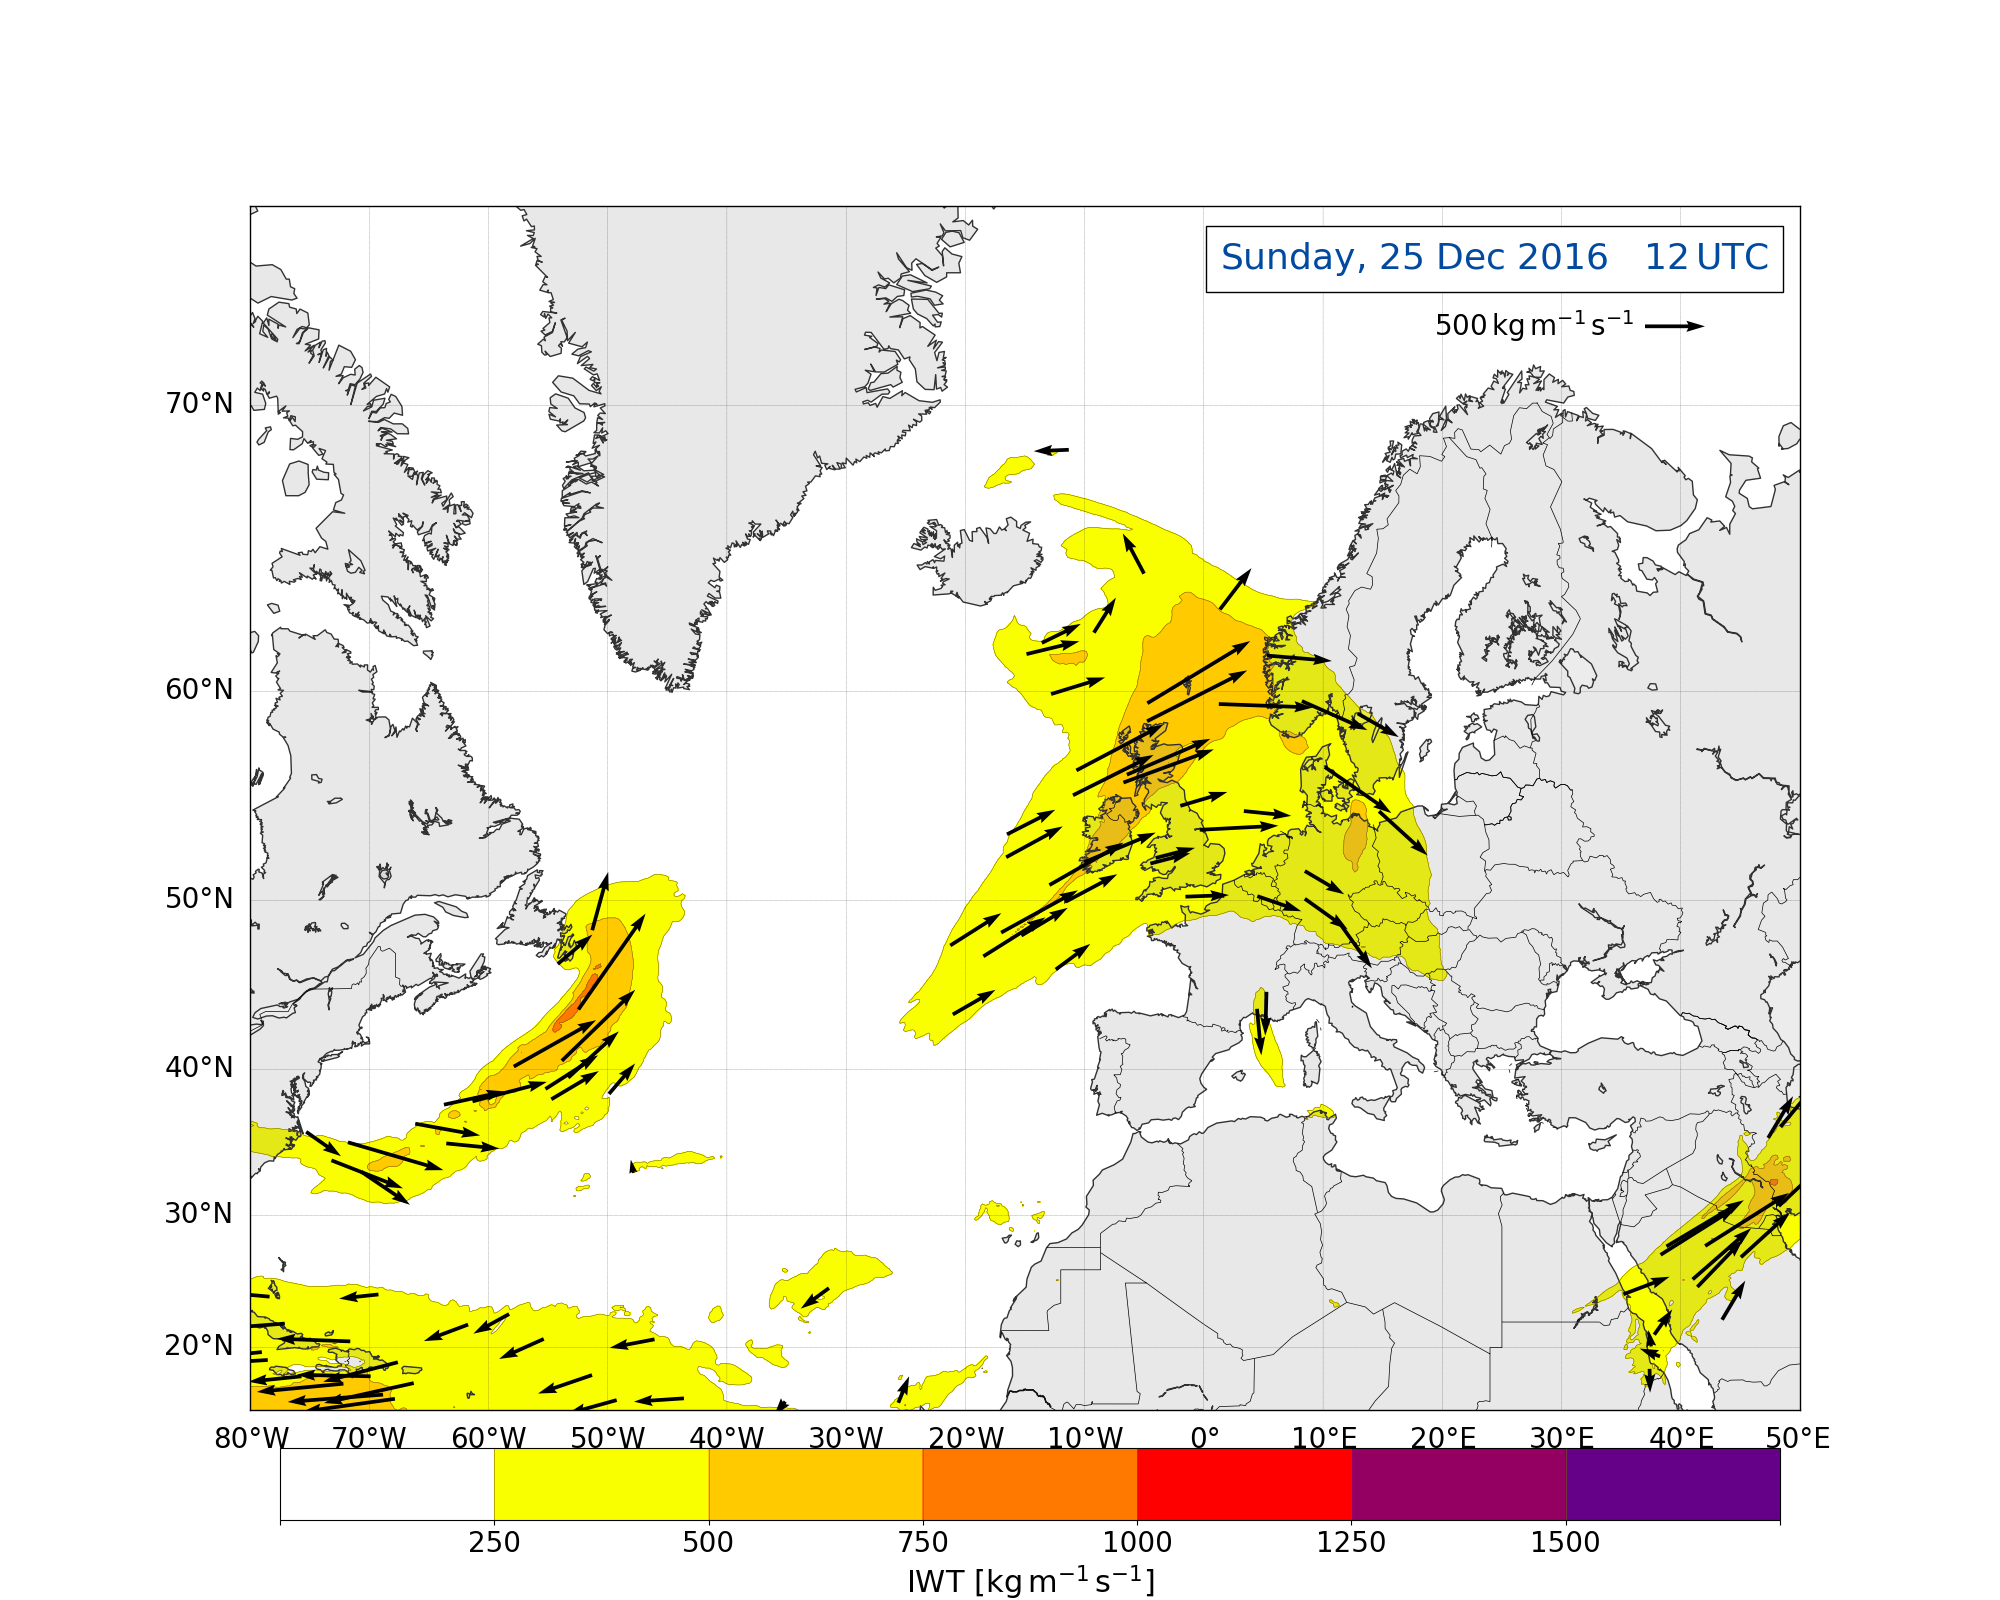
\includegraphics[trim={4.2cm 0cm 4.3cm 36.8cm},clip,
		width=\textwidth]{./fig_Atm_Riv/20161225_12}
	\end{subfigure}
\end{figure}
%
\begin{figure}\ContinuedFloat
	\centering
	%%%%%% 22/12
	\begin{subfigure}[b]{0.49\textwidth}
		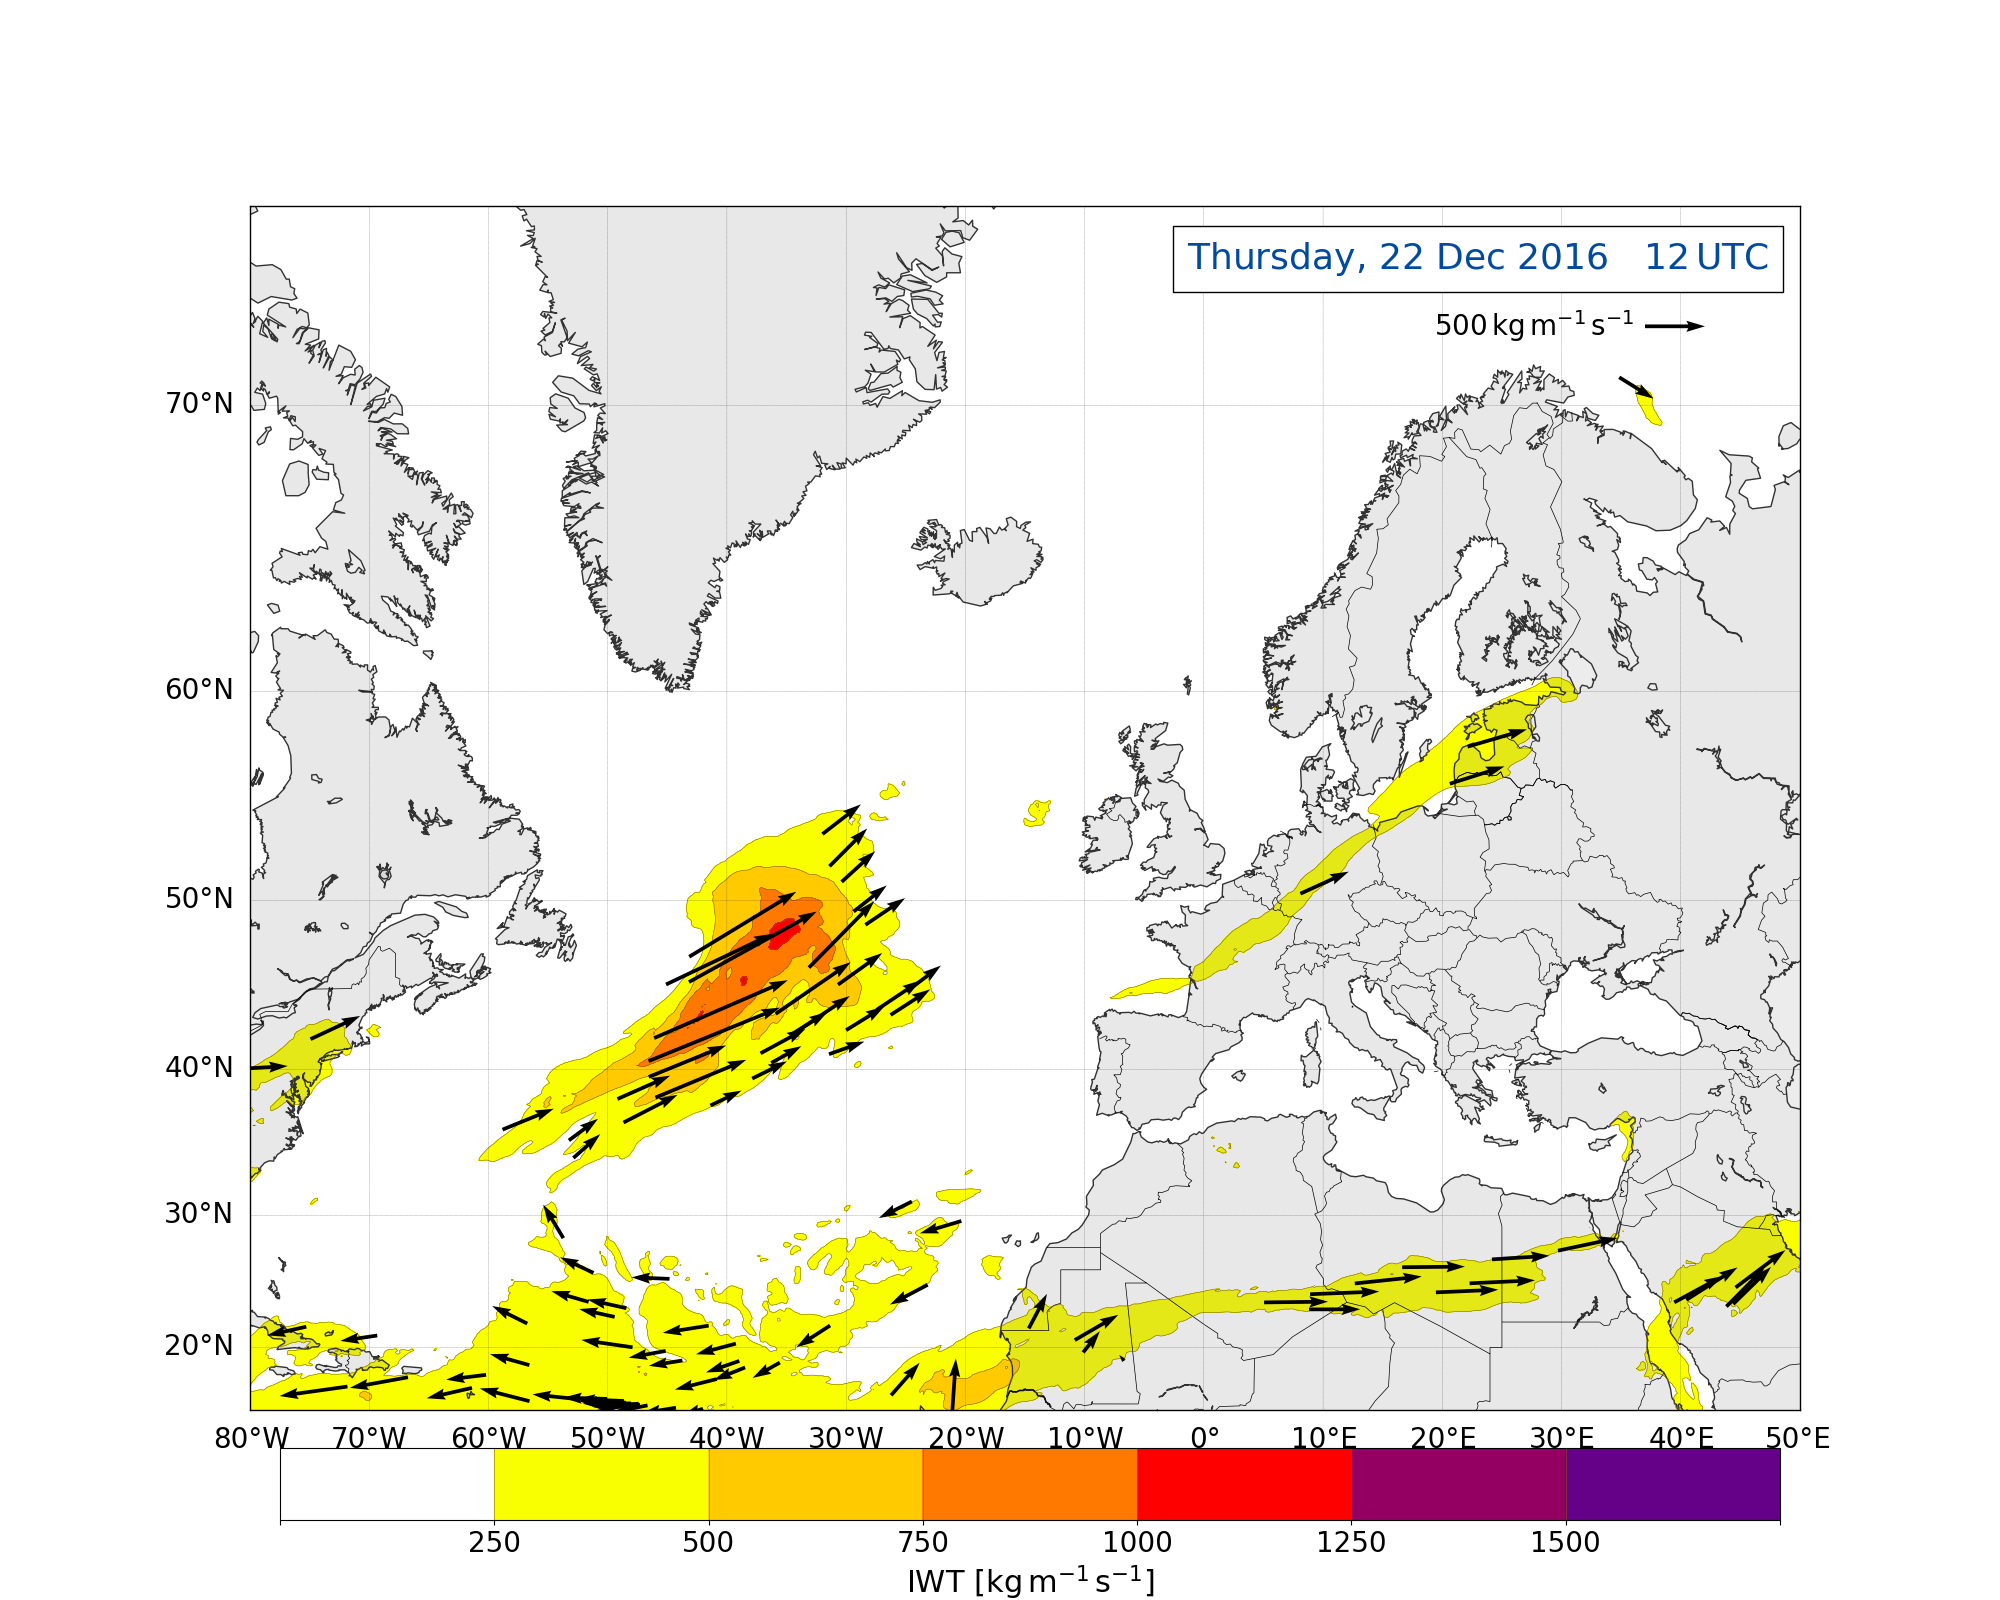
\includegraphics[trim={4.2cm 3.9cm 4.3cm 5.1cm},clip,
		width=\textwidth]{./fig_Atm_Riv/20161222_12}
		\caption{}\label{fig:AR22}
		%\label{fig:sfc2100}
	\end{subfigure}
	%%%%%% 23/12
	\begin{subfigure}[b]{0.49\textwidth}
		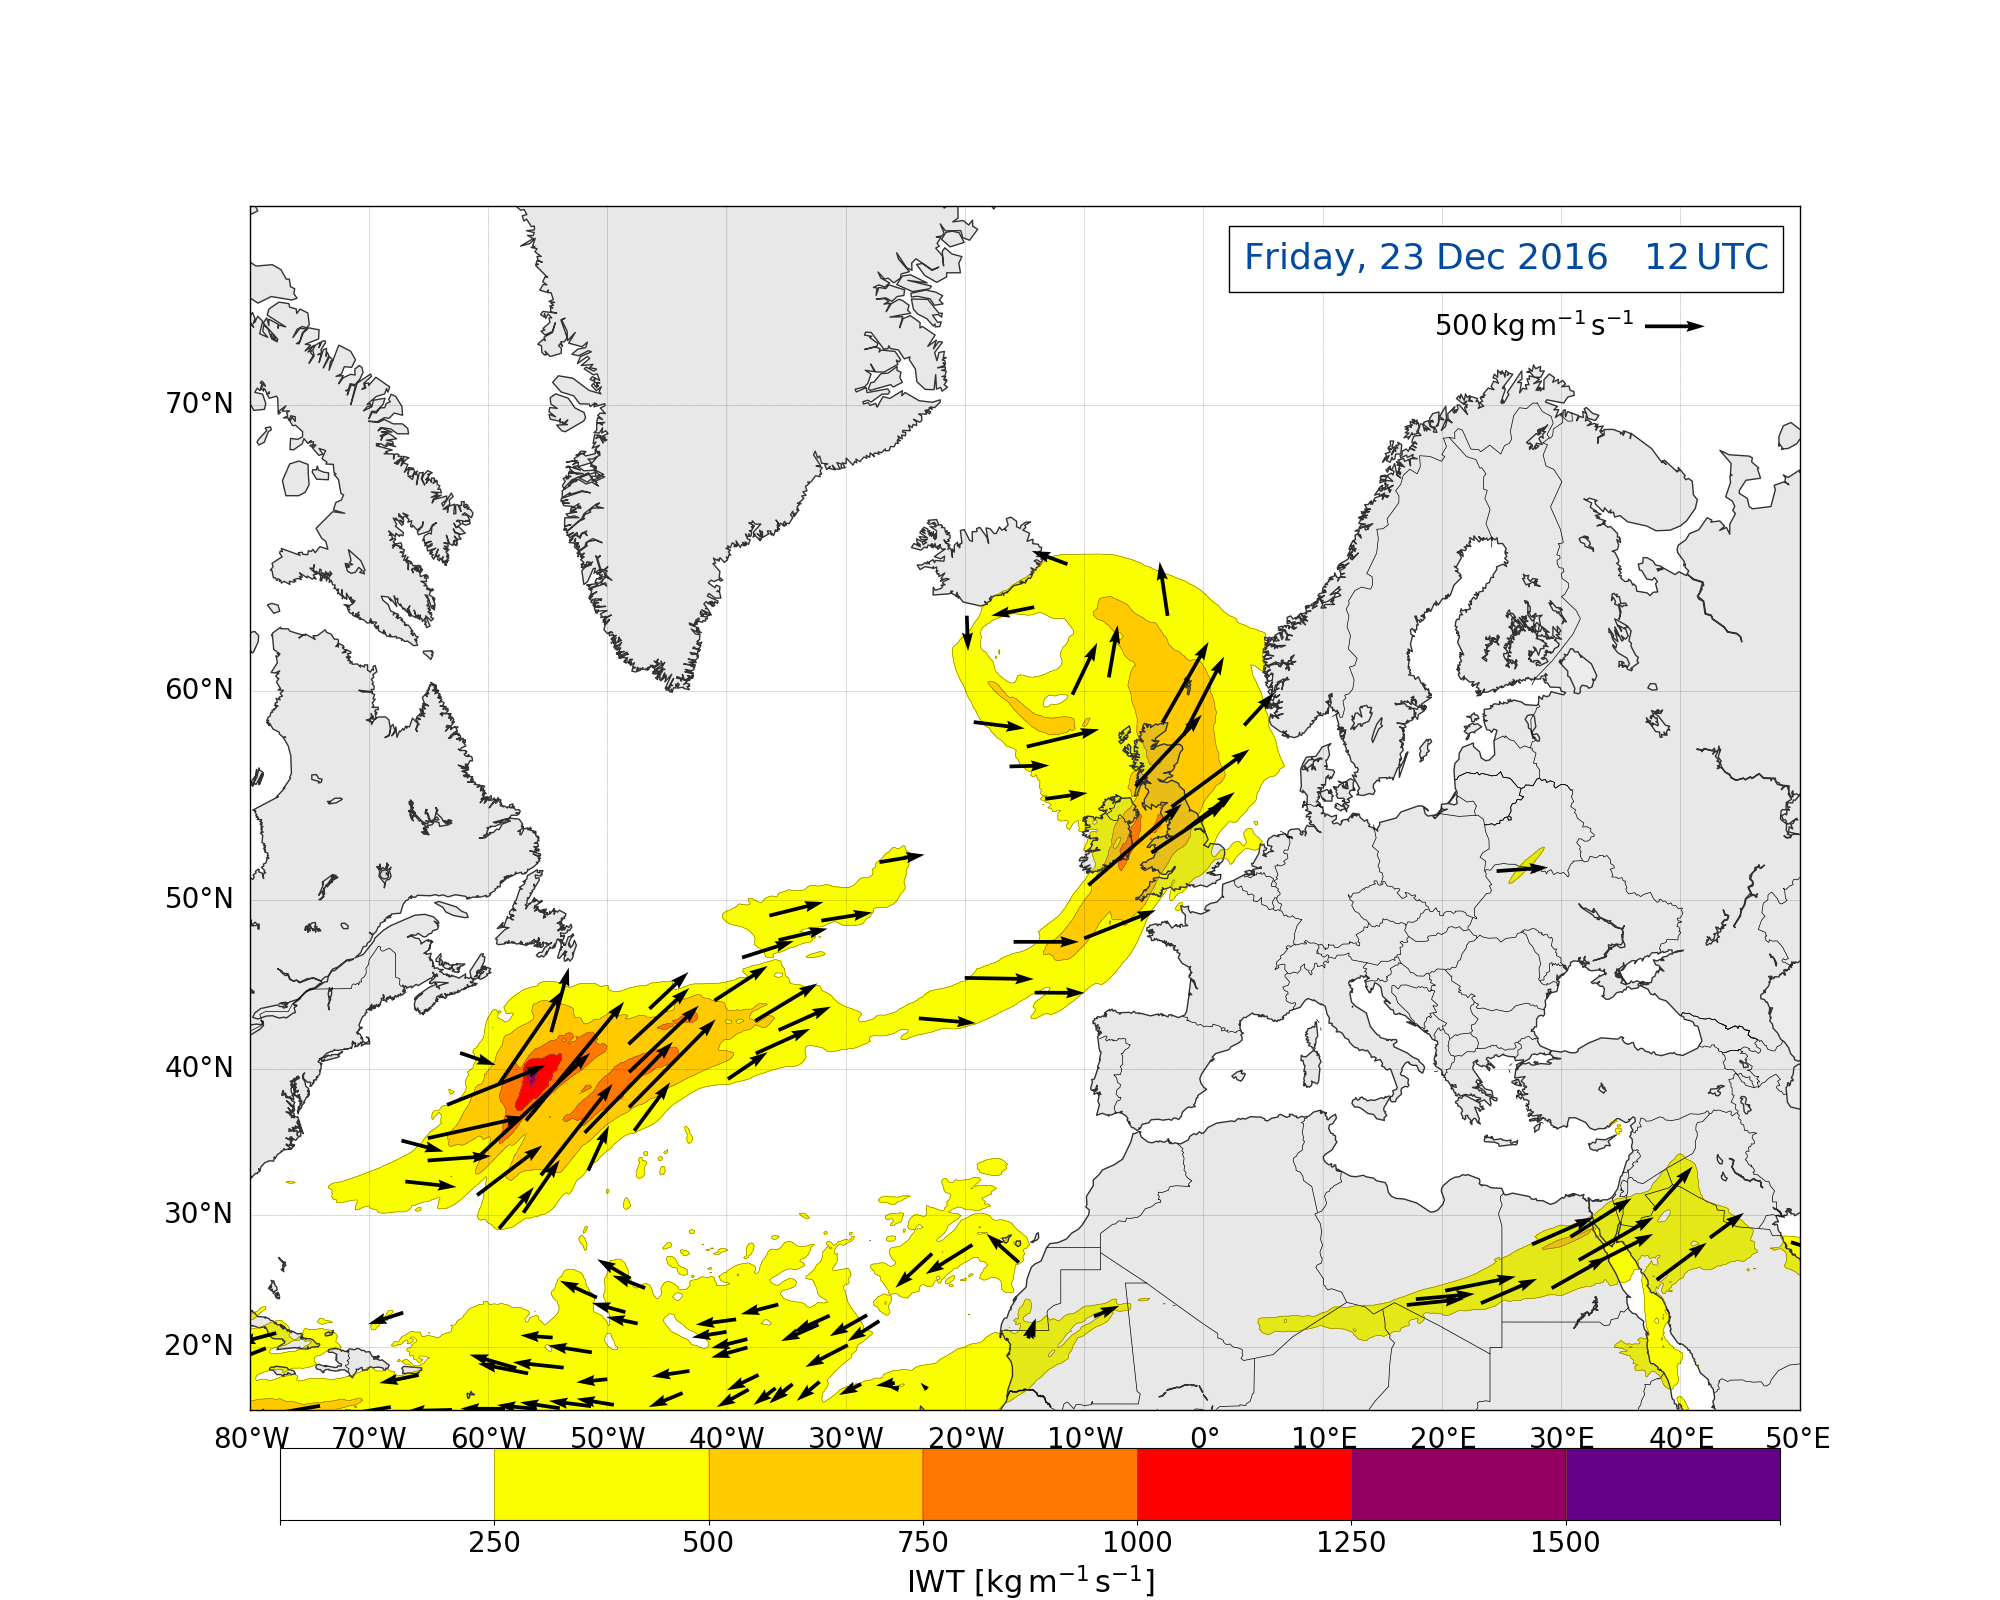
\includegraphics[trim={4.2cm 3.9cm 4.3cm 5.1cm},clip,
		width=\textwidth]{./fig_Atm_Riv/20161223_12}
		\caption{}\label{fig:AR23}
	\end{subfigure}
	%%%%%% 24/12
	\begin{subfigure}[b]{0.49\textwidth}
		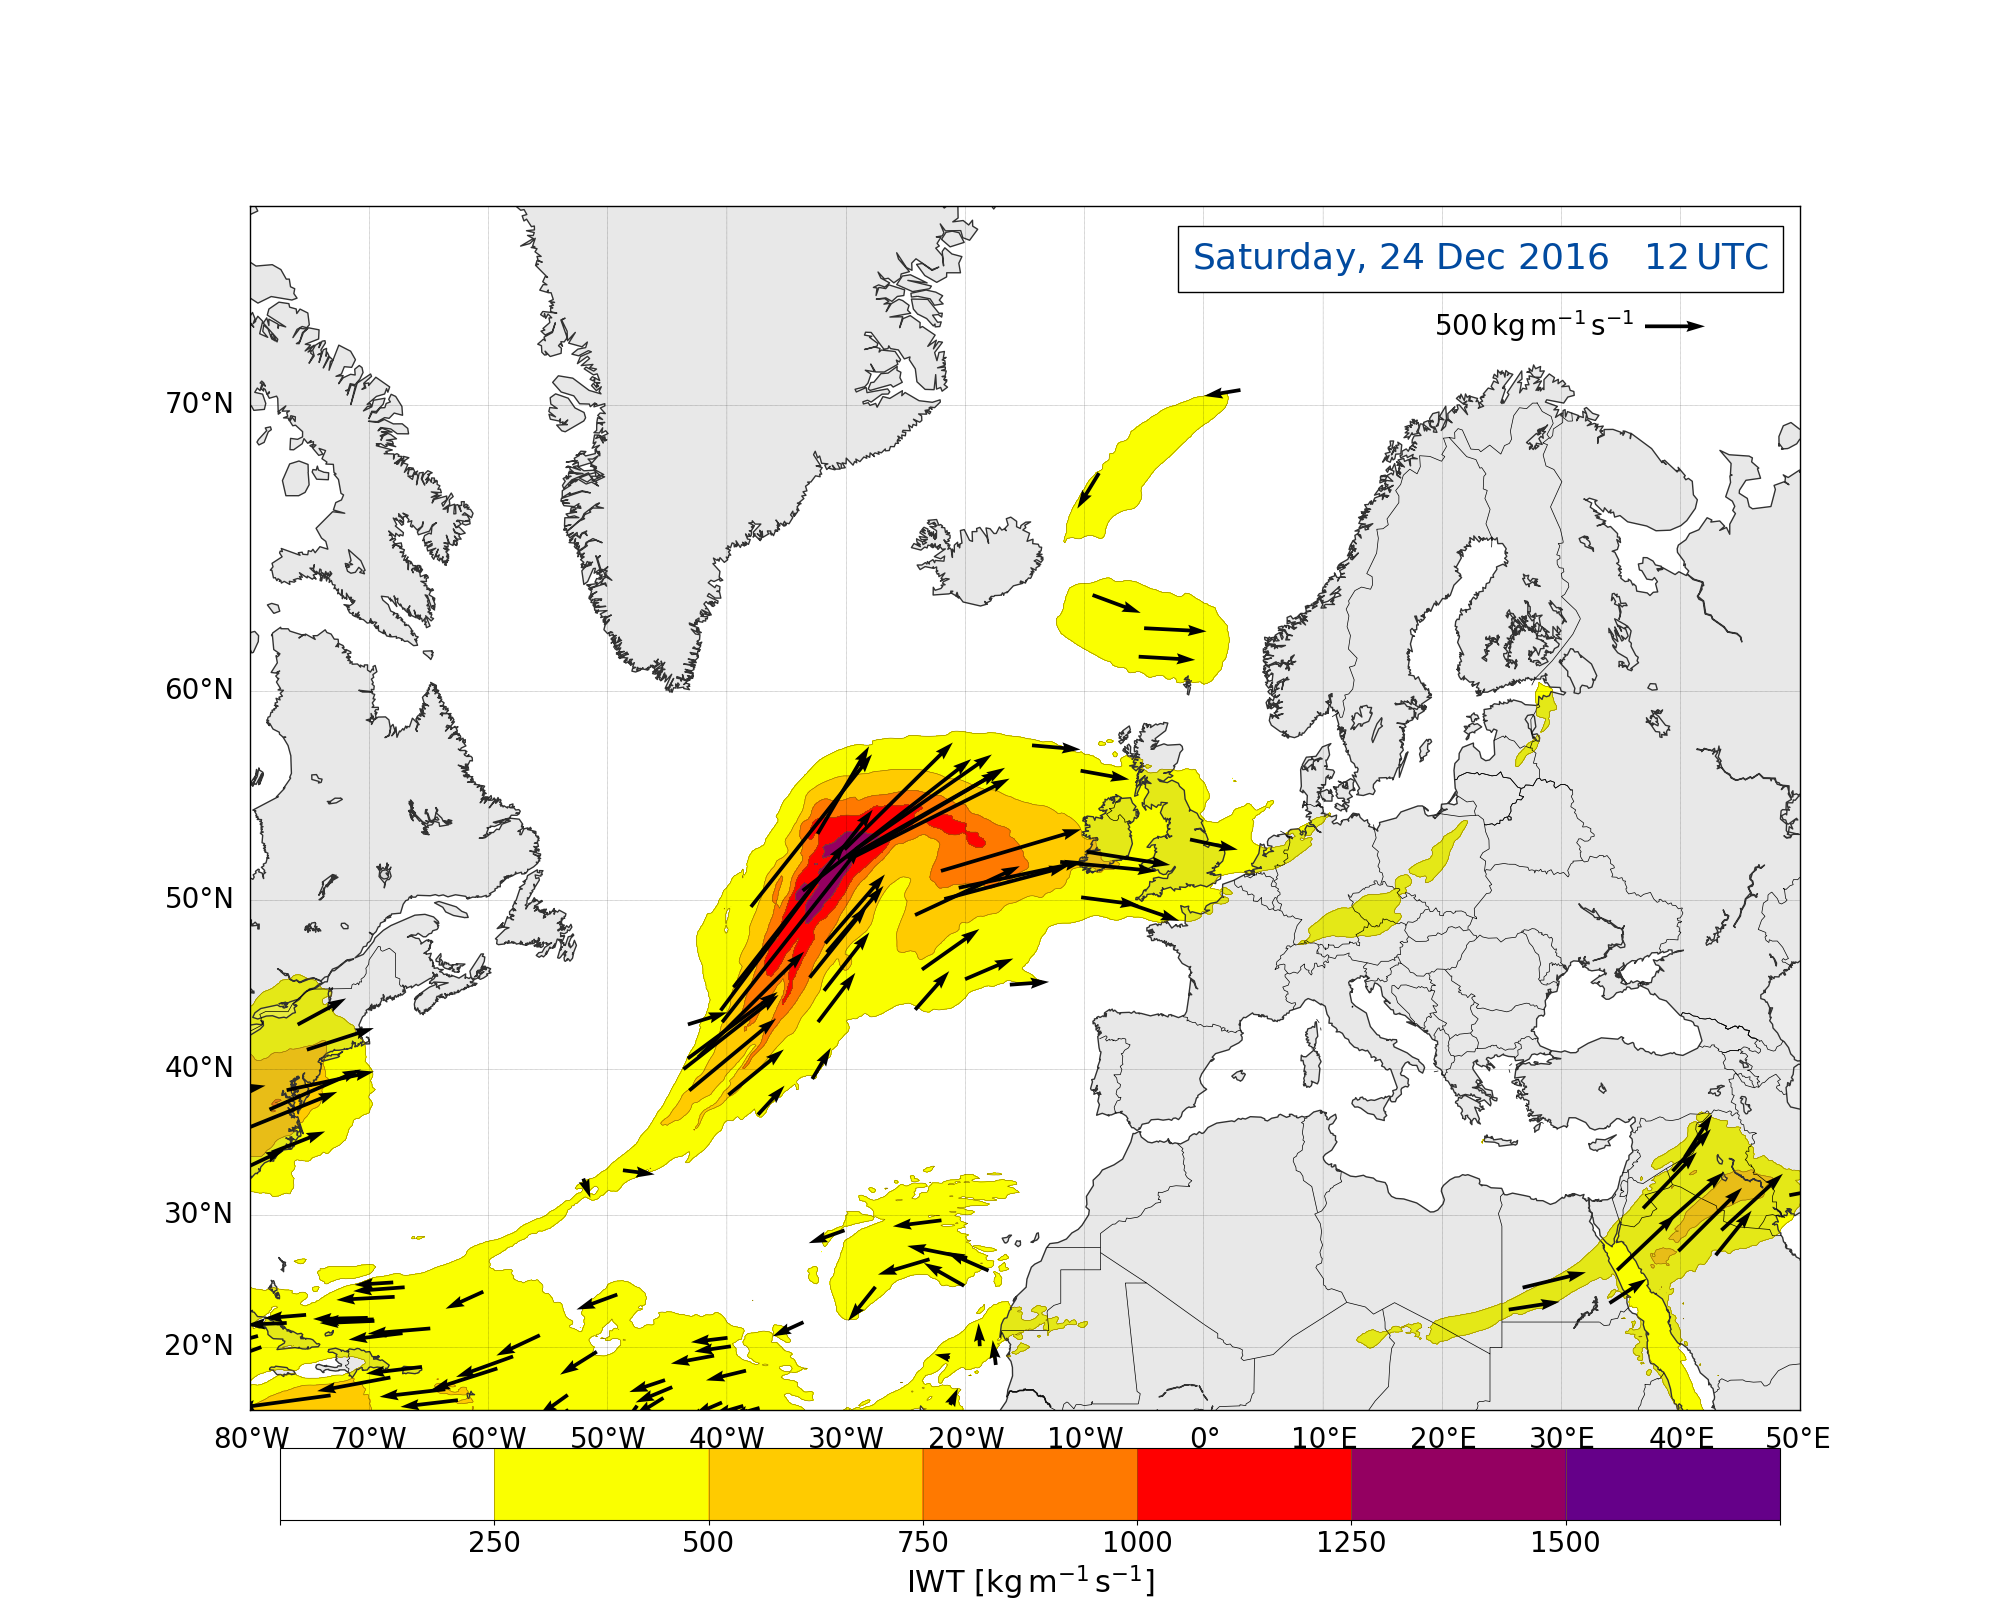
\includegraphics[trim={4.2cm 3.9cm 4.3cm 5.1cm},clip,
		width=\textwidth]{./fig_Atm_Riv/20161224_12}
		\caption{}\label{fig:AR24}
	\end{subfigure}
	%%%%%% 25/12
	\begin{subfigure}[b]{0.49\textwidth}
		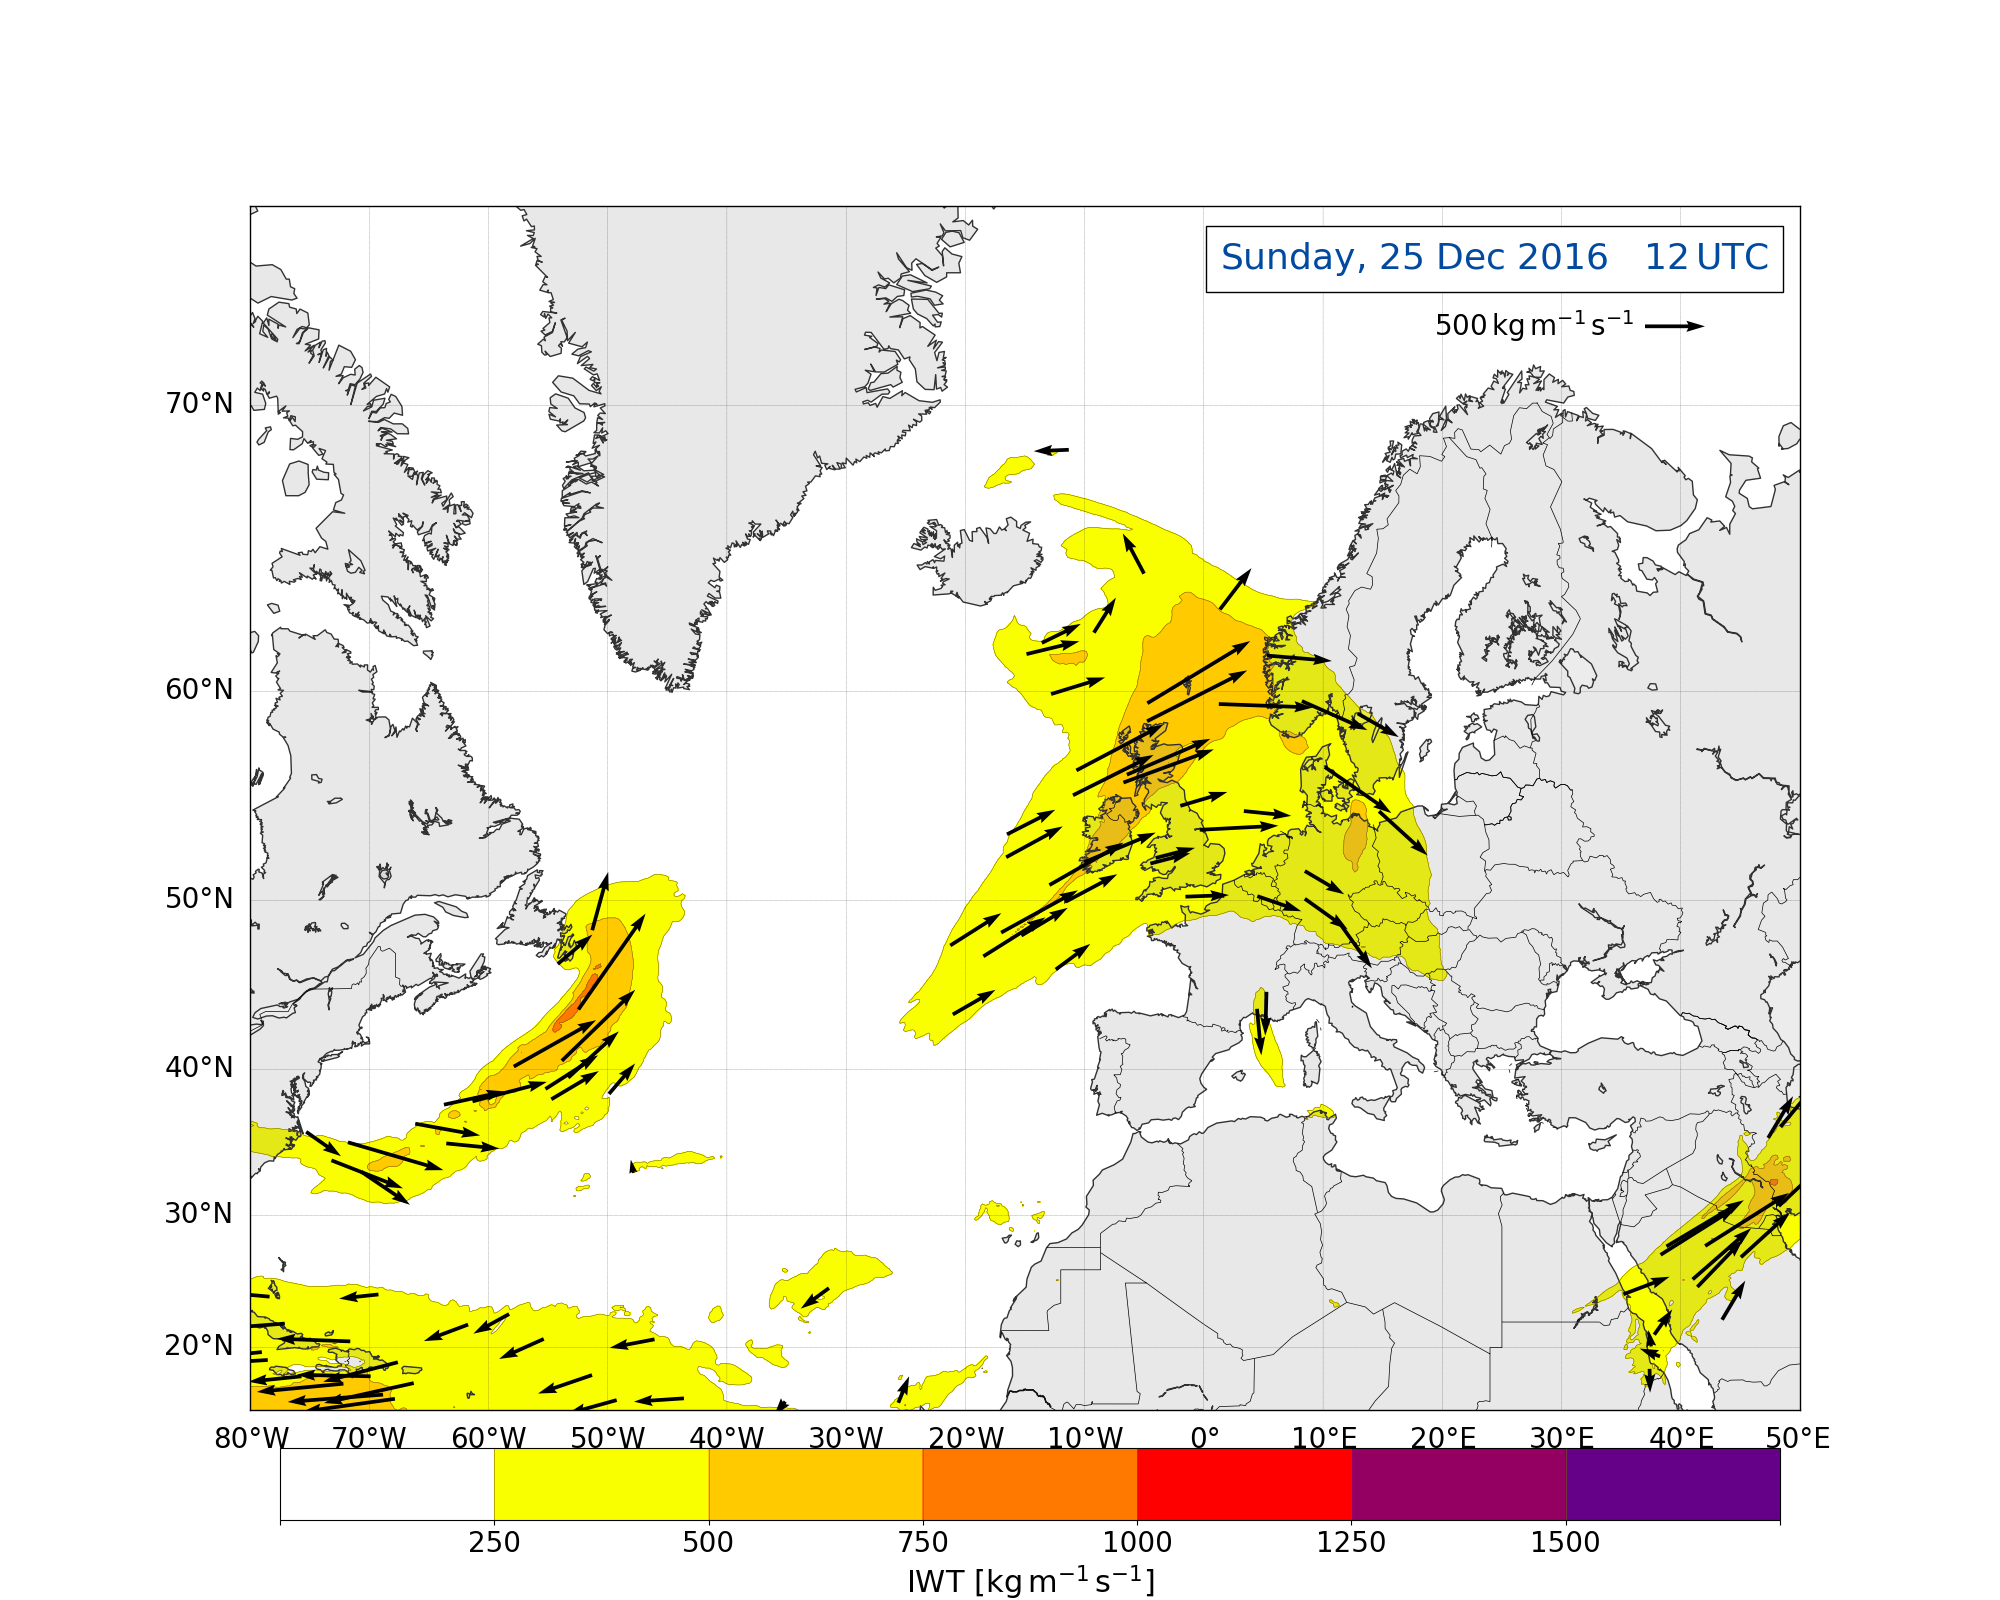
\includegraphics[trim={4.2cm 3.9cm 4.3cm 5.1cm},clip,
		width=\textwidth]{./fig_Atm_Riv/20161225_12}
		\caption{}\label{fig:AR25}
	\end{subfigure}
	%	\centering
	%%%%%% 26/12
	\begin{subfigure}[b]{0.49\textwidth}
		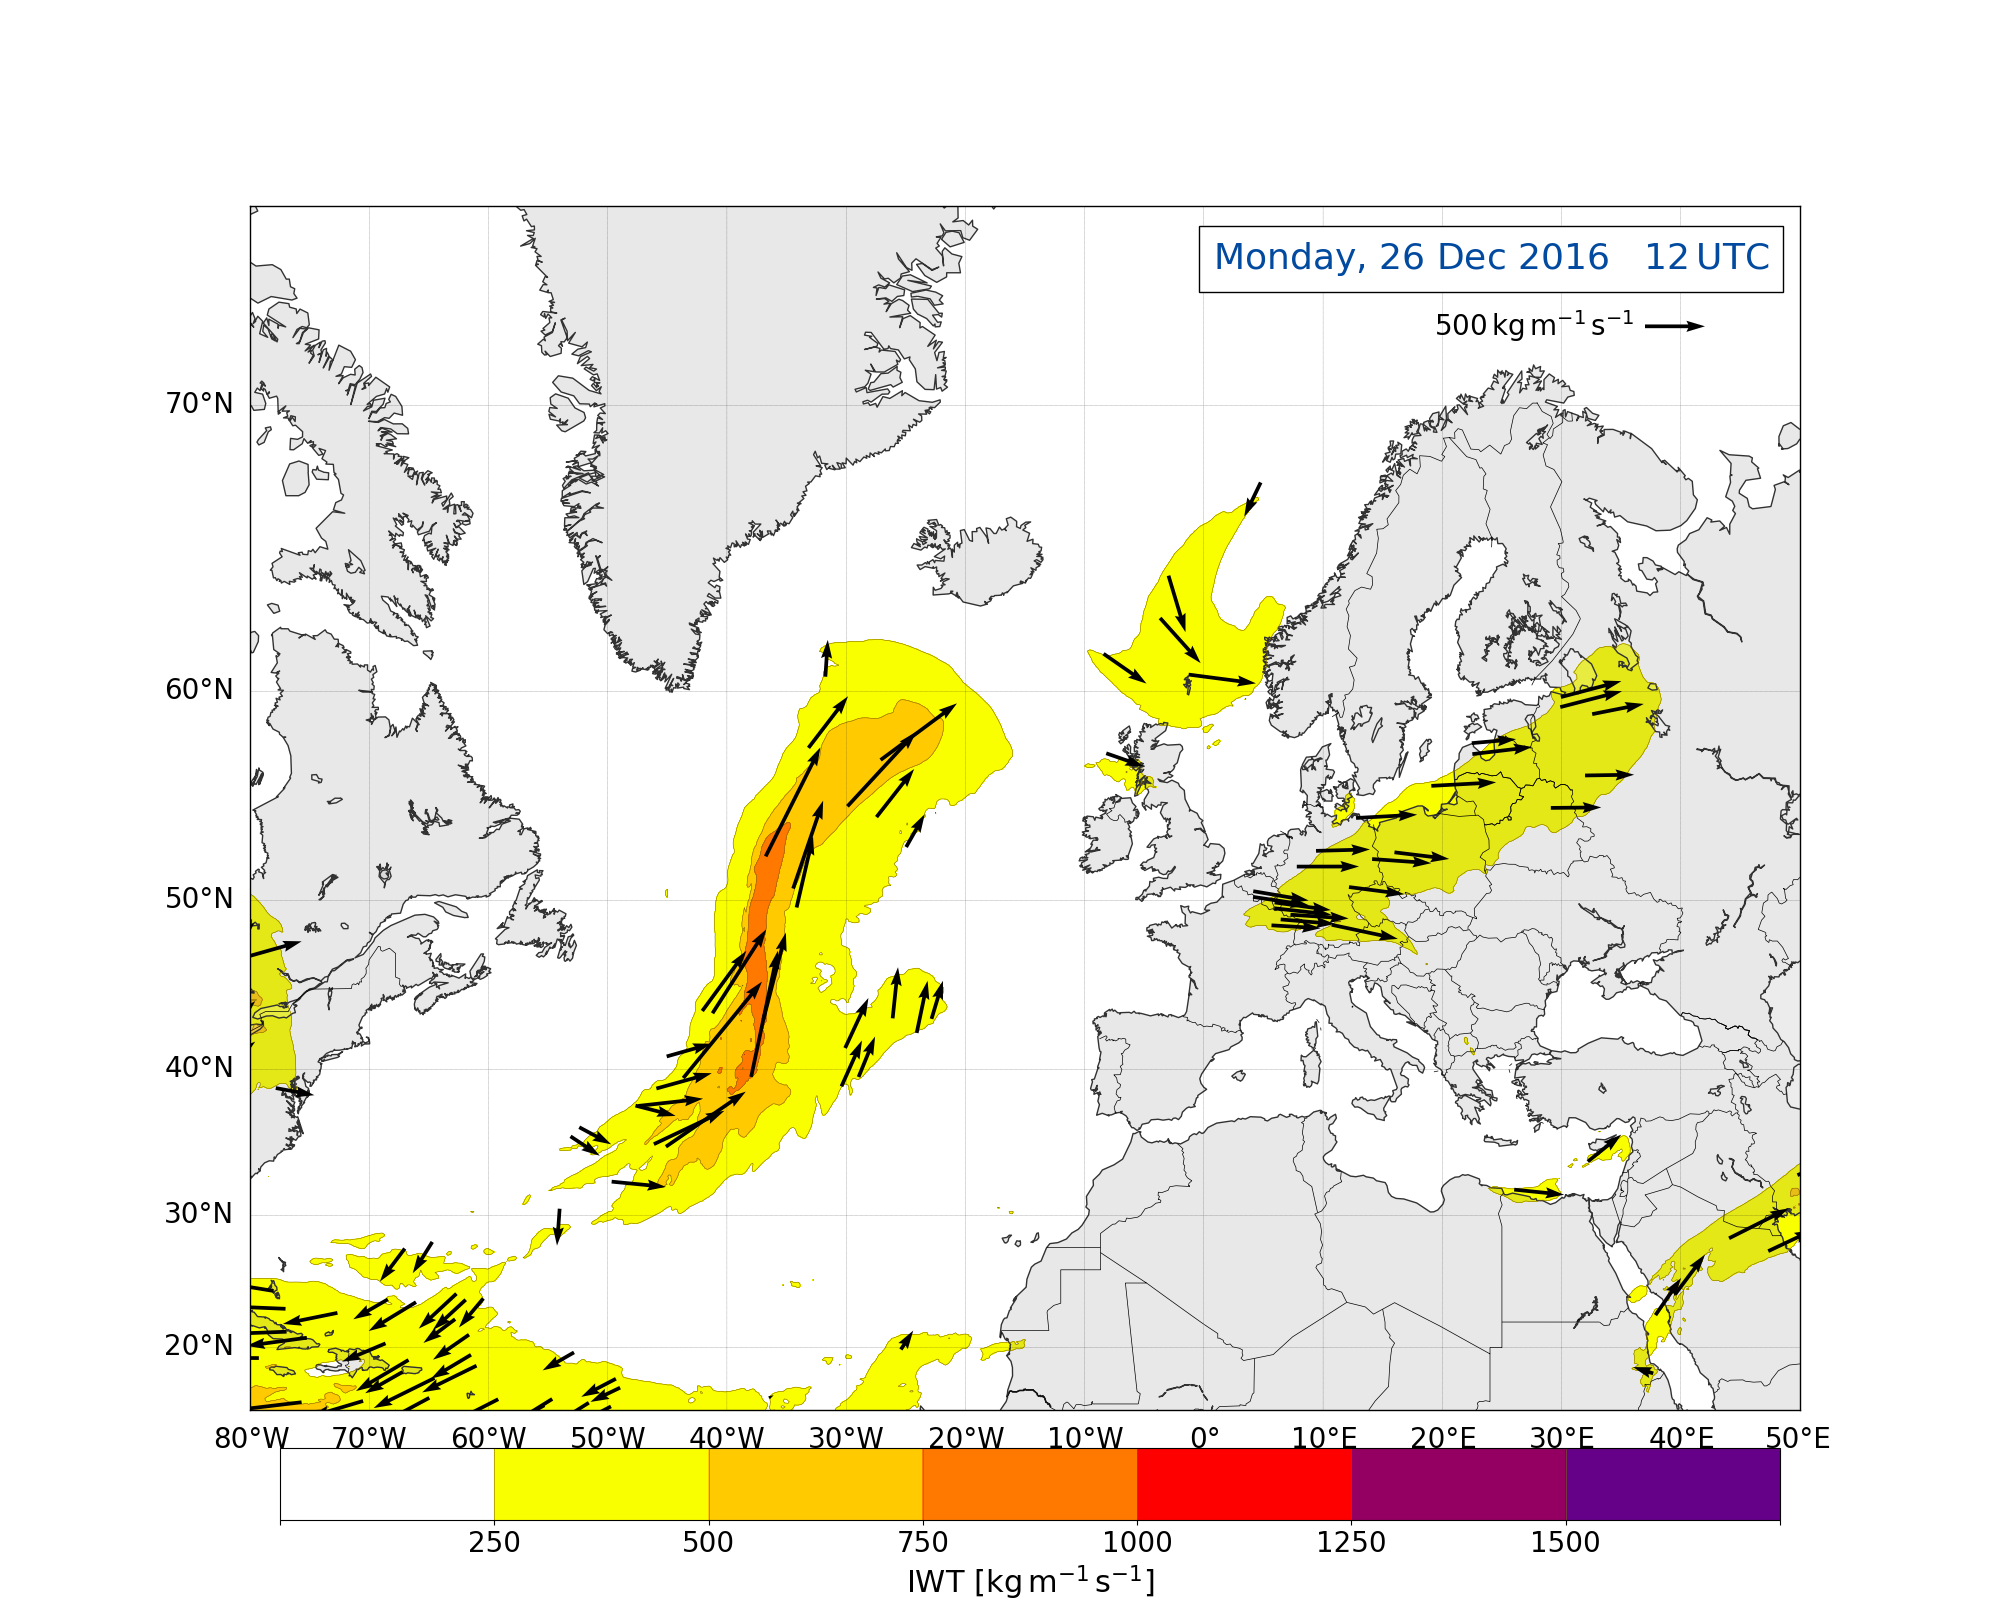
\includegraphics[trim={4.2cm 3.9cm 4.3cm 5.1cm},clip,
		width=\textwidth]{./fig_Atm_Riv/20161226_12}
		\caption{}\label{fig:AR26}
	\end{subfigure}
	%%%%%% 27/12
	\begin{subfigure}[b]{0.49\textwidth}
		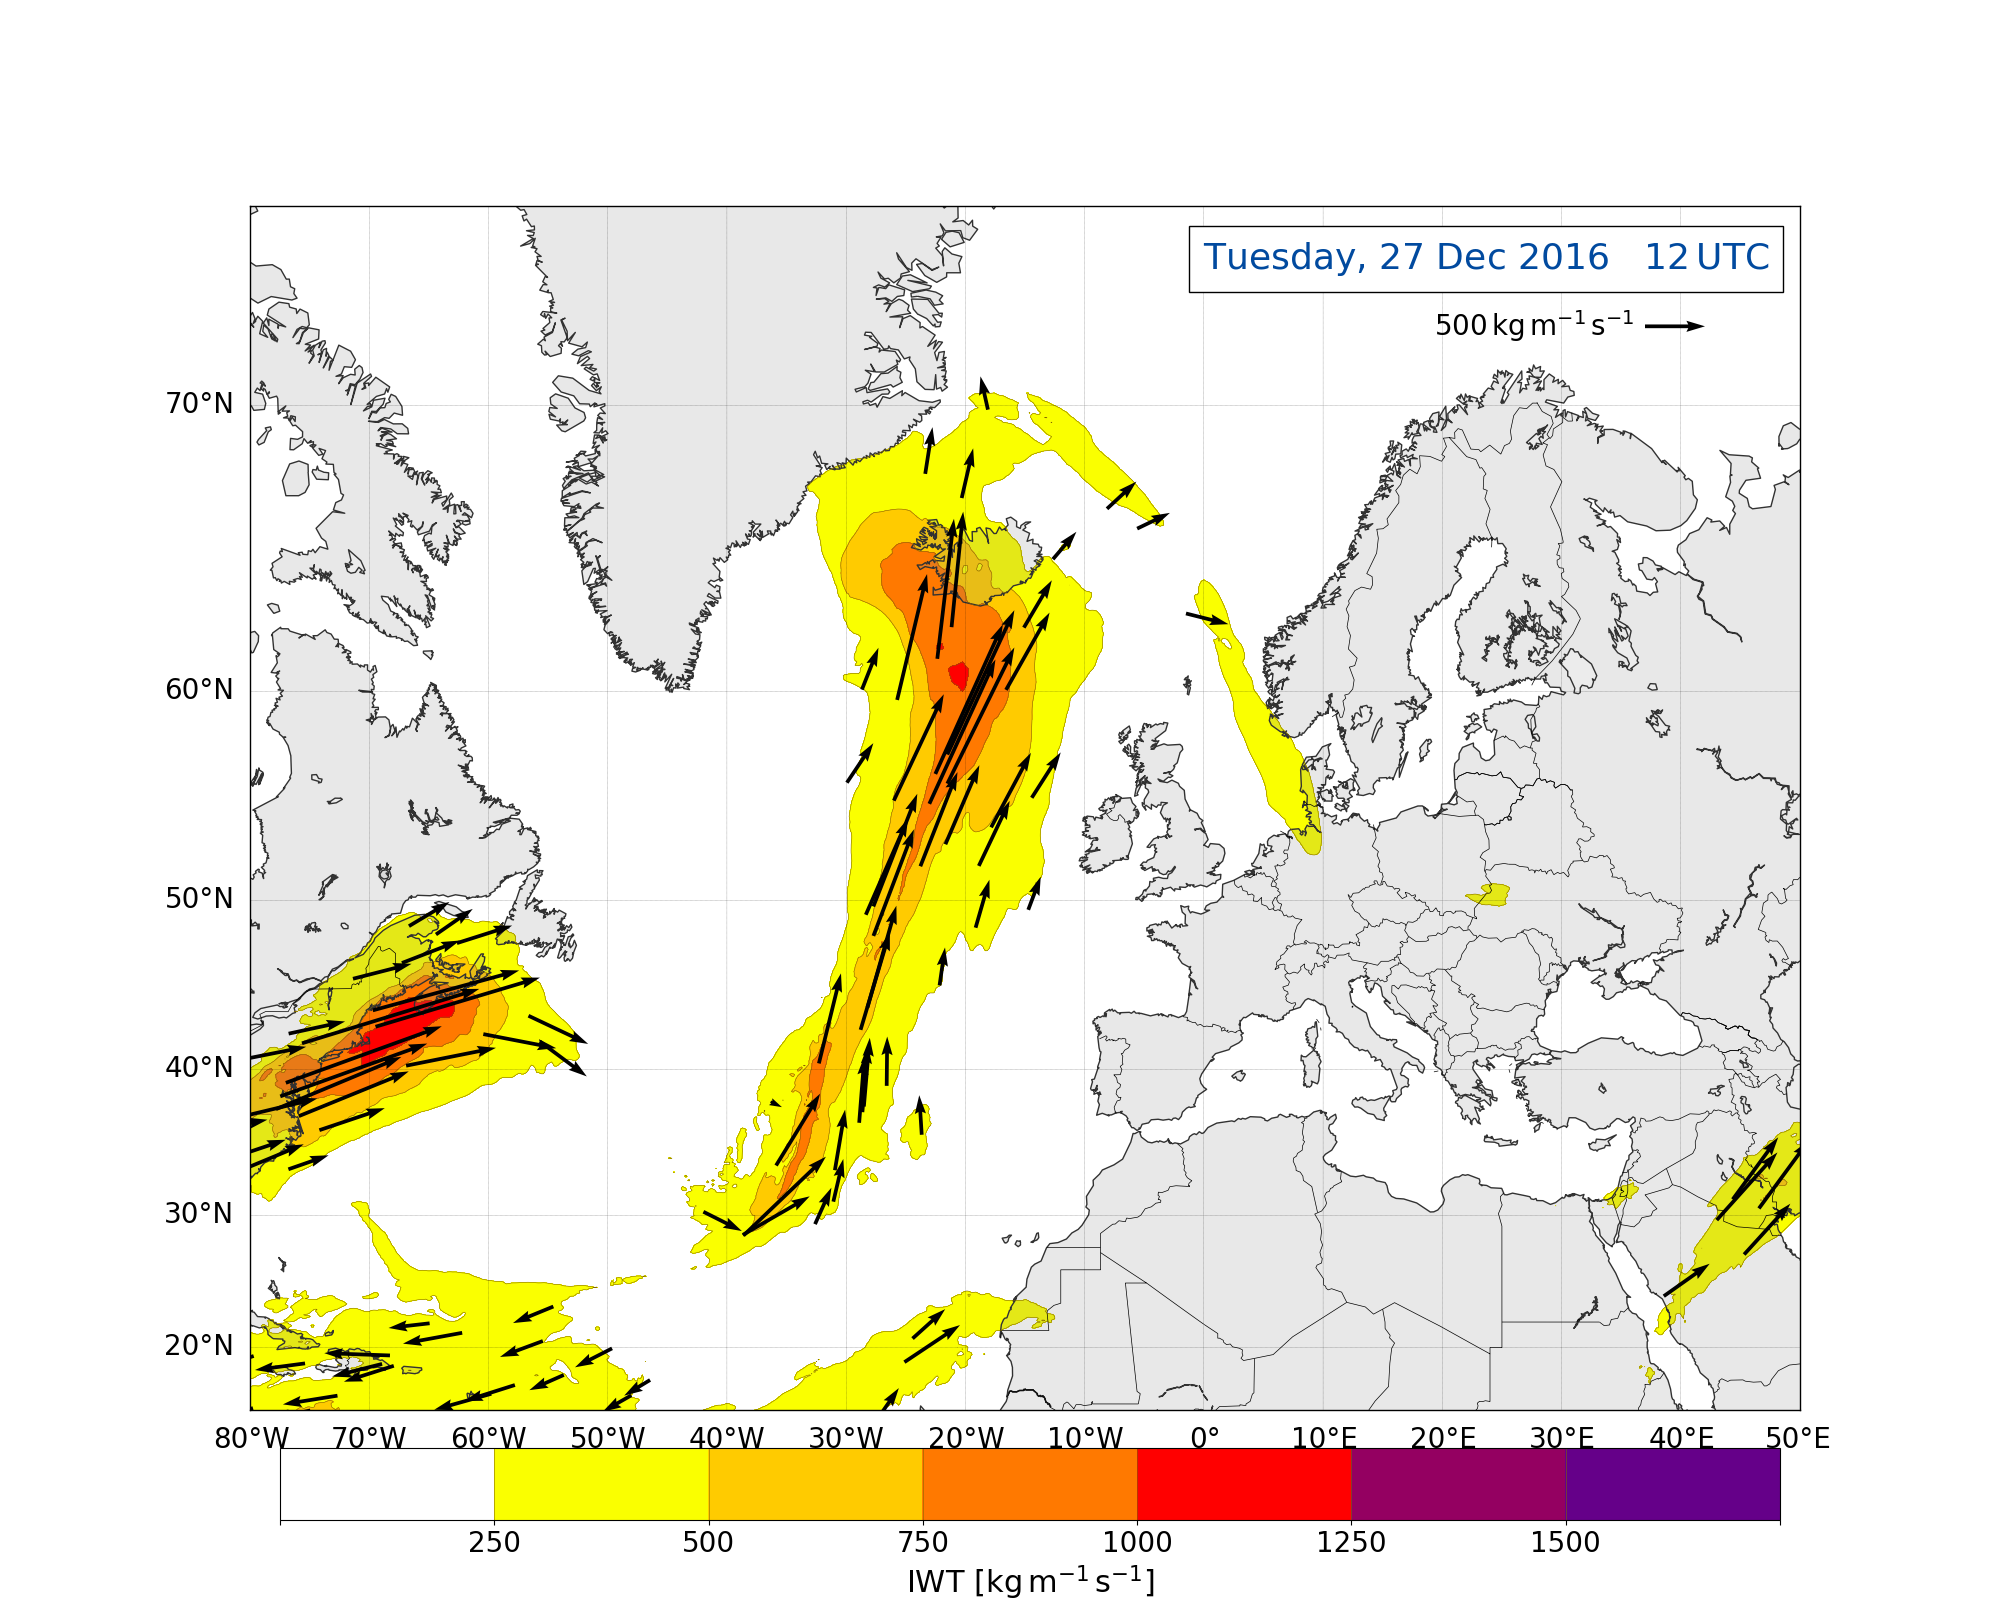
\includegraphics[trim={4.2cm 3.9cm 4.3cm 5.1cm},clip,
		width=\textwidth]{./fig_Atm_Riv/20161227_12}
		\caption{}\label{fig:AR27}
	\end{subfigure}
	%%%%%% label
	\begin{subfigure}[b]{\textwidth}
		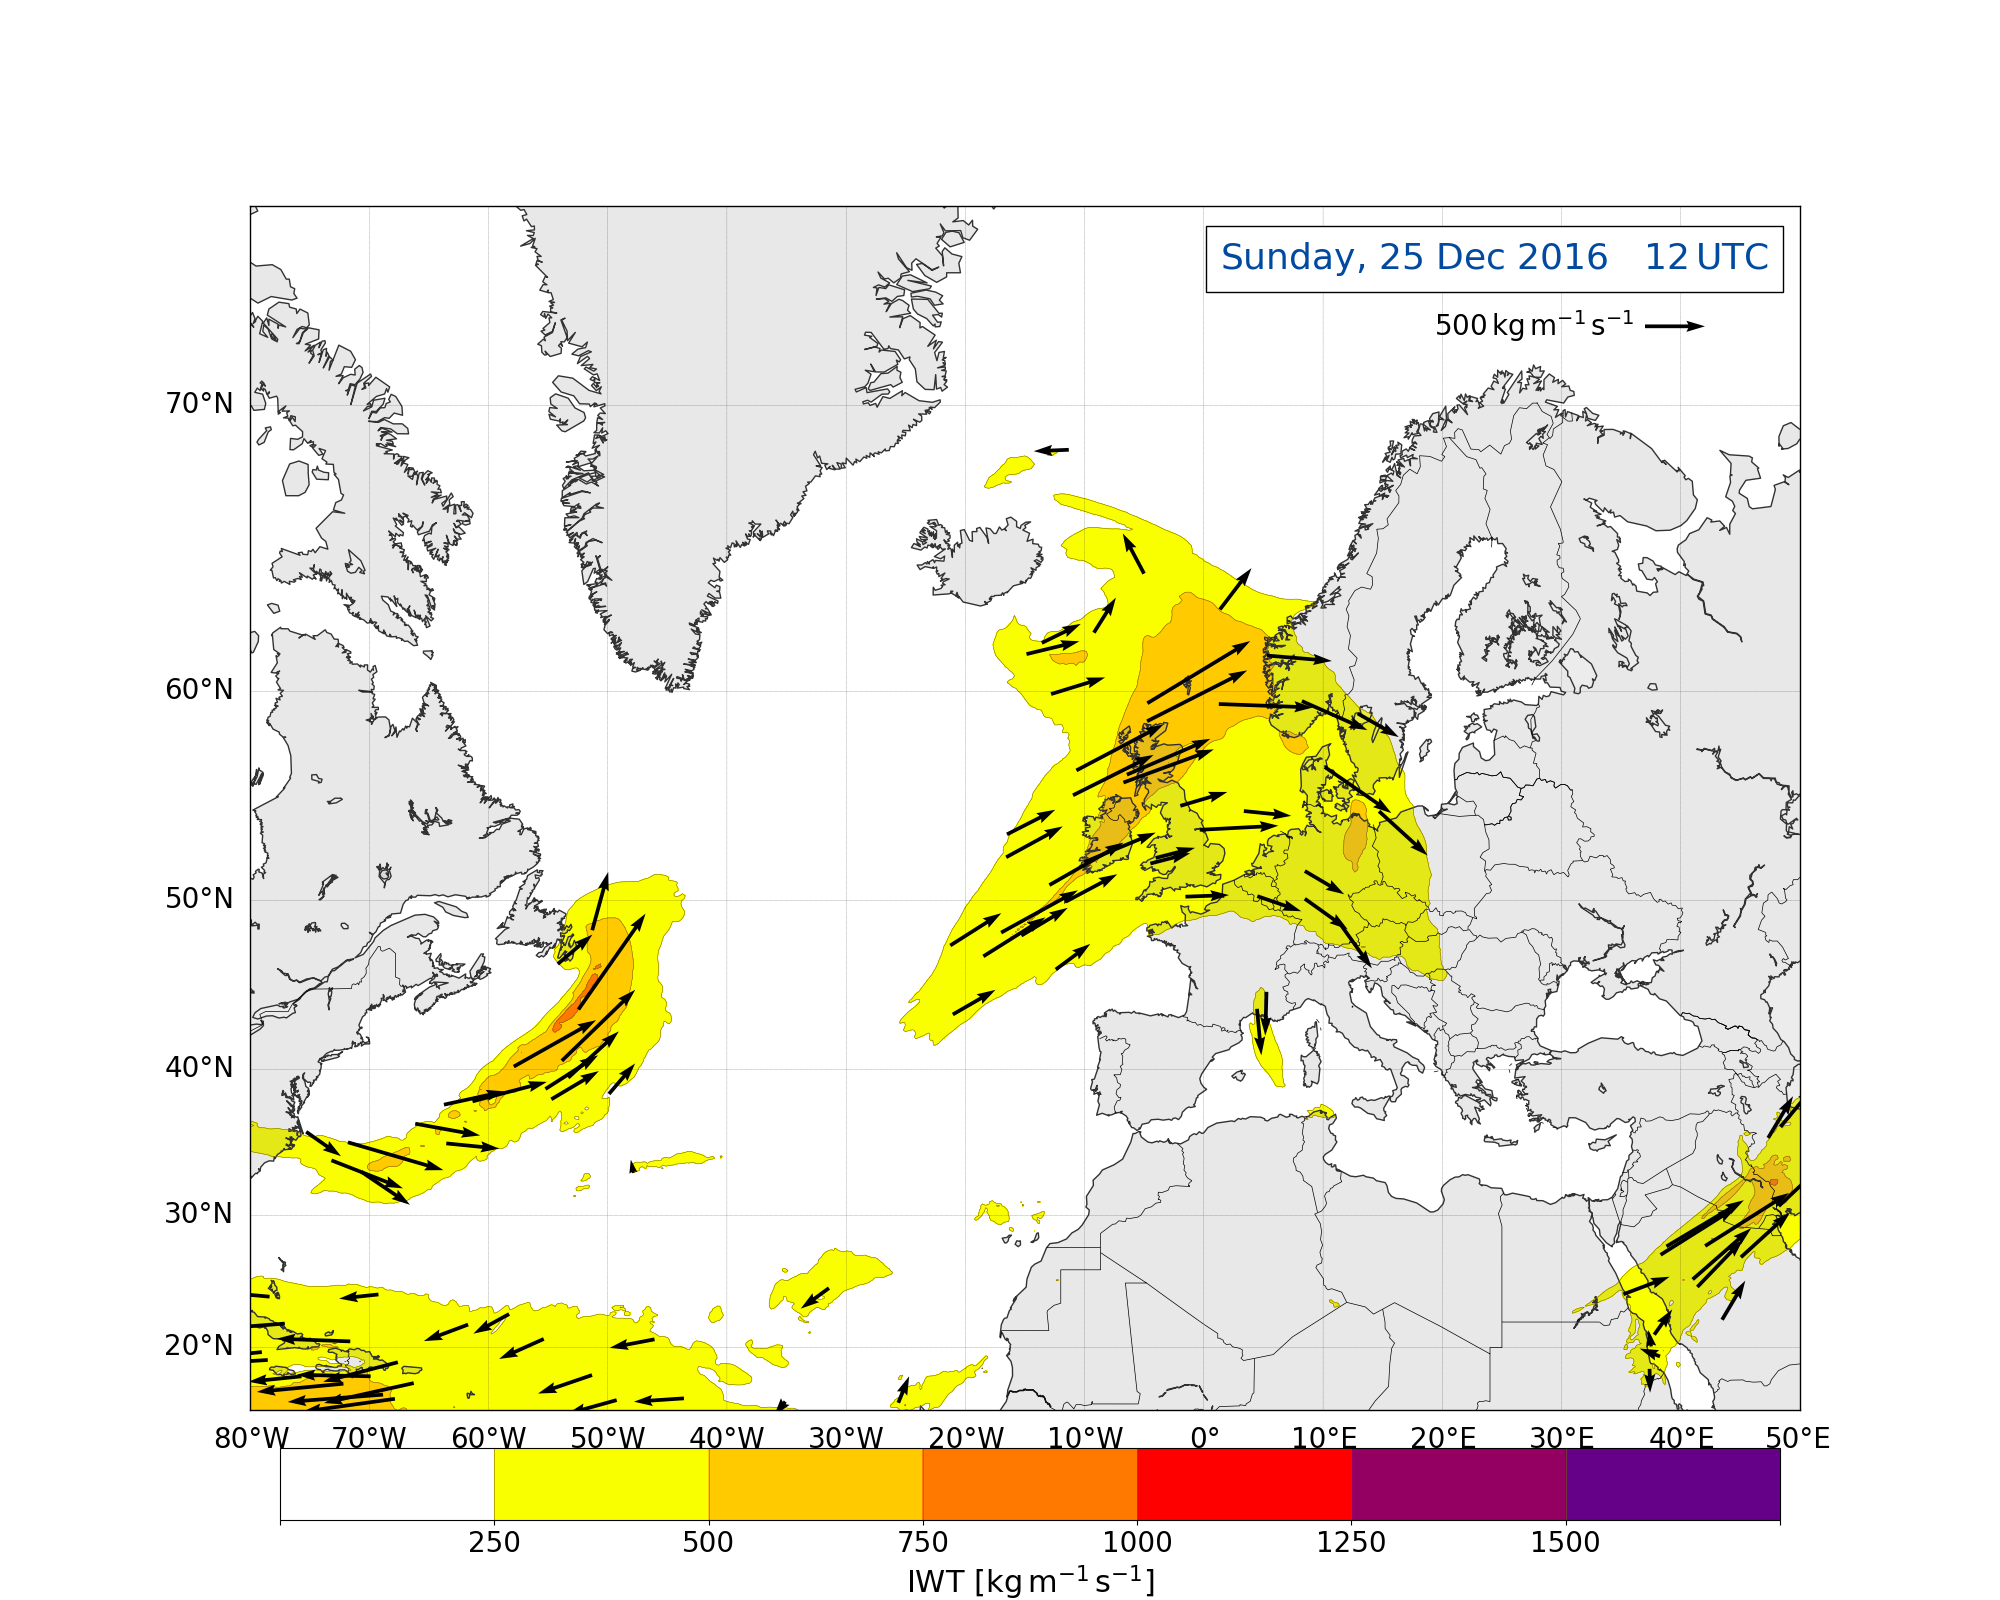
\includegraphics[trim={4.2cm 0cm 4.3cm 36.8cm},clip,
		width=\textwidth]{./fig_Atm_Riv/20161225_12}
	\end{subfigure}
	\caption{Atmospheric river analysis map, data from ECMWF. During \SIrange{20}{27}{\dec}. IVT, shaded according to the colour bar [\SI{}{\IVT}]. Vectors, indicating the direction and magnitude of the IVT. }\label{fig:AtmRiv}
\end{figure}
%%%%%%%%%%%%%%%%%%%%%%%%%%%%%%%%%%%%%%%%%%%%%%%%%%%%%%%%%%%%%%%%%%%%%%%%%%
An atmospheric river (AR) is a filament structure of intense moisture transport from the tropics to higher latitudes. 
Heavy precipitation can be associated with it, because the air is warm and moist. This can often be observed at mountain ranges at west coasts such as in Norway \textcolor{red}{include reference here}. Due to orographic lifting will the moisture be released and follow high amounts of precipitation.  
\\
An atmospheric river is characterised if the integrated vapour transport shows values higher than \SI{250}{\IVT} and is a continuous region larger than \SI{2000}{\km} \citep{rutz_climatological_2014}.
The integrated vapour transport (IVT) was calculated from the ECMWF data as followed:
\begin{align}
IVT = \frac{1}{g} \int\limits_{p_{sfc}}^{\SI{100}{\hPa}} q \mathbf{V} dp \qquad [\SI{}{\IVT}]
\label{eq:IVT}
\end{align} 
where $g$ is the standard gravity, $q$ the specific humidity, and $\mathbf{V}$ the total wind vector at each pressure level $p$. The numerical, trapezoidal integration is performed by using data from the surface pressure $p_{sfc}$ to \SI{850}{\hPa} in \SI{50}{\hPa} intervals and from \SIrange{700}{100}{\hPa} in \SI{100}{\hPa} intervals.
\\
\Cref{fig:AtmRiv} shows coloured contours of the integrated vapour transport (IVT) in \SI{}{\IVT}, where warmer colours indicate higher IVT. Stream vectors indicate the direction and intensity of the IVT flow.

%%% Atmospheric river maps %%%%%%%%%%%%%%%%%%%%%%%%%%%%%%%%%%%%%
%% !TeX spellcheck = en_GB
\begin{figure}[h!]
	\centering
	%%%%%% 20/12
	\begin{subfigure}[b]{0.49\textwidth}
		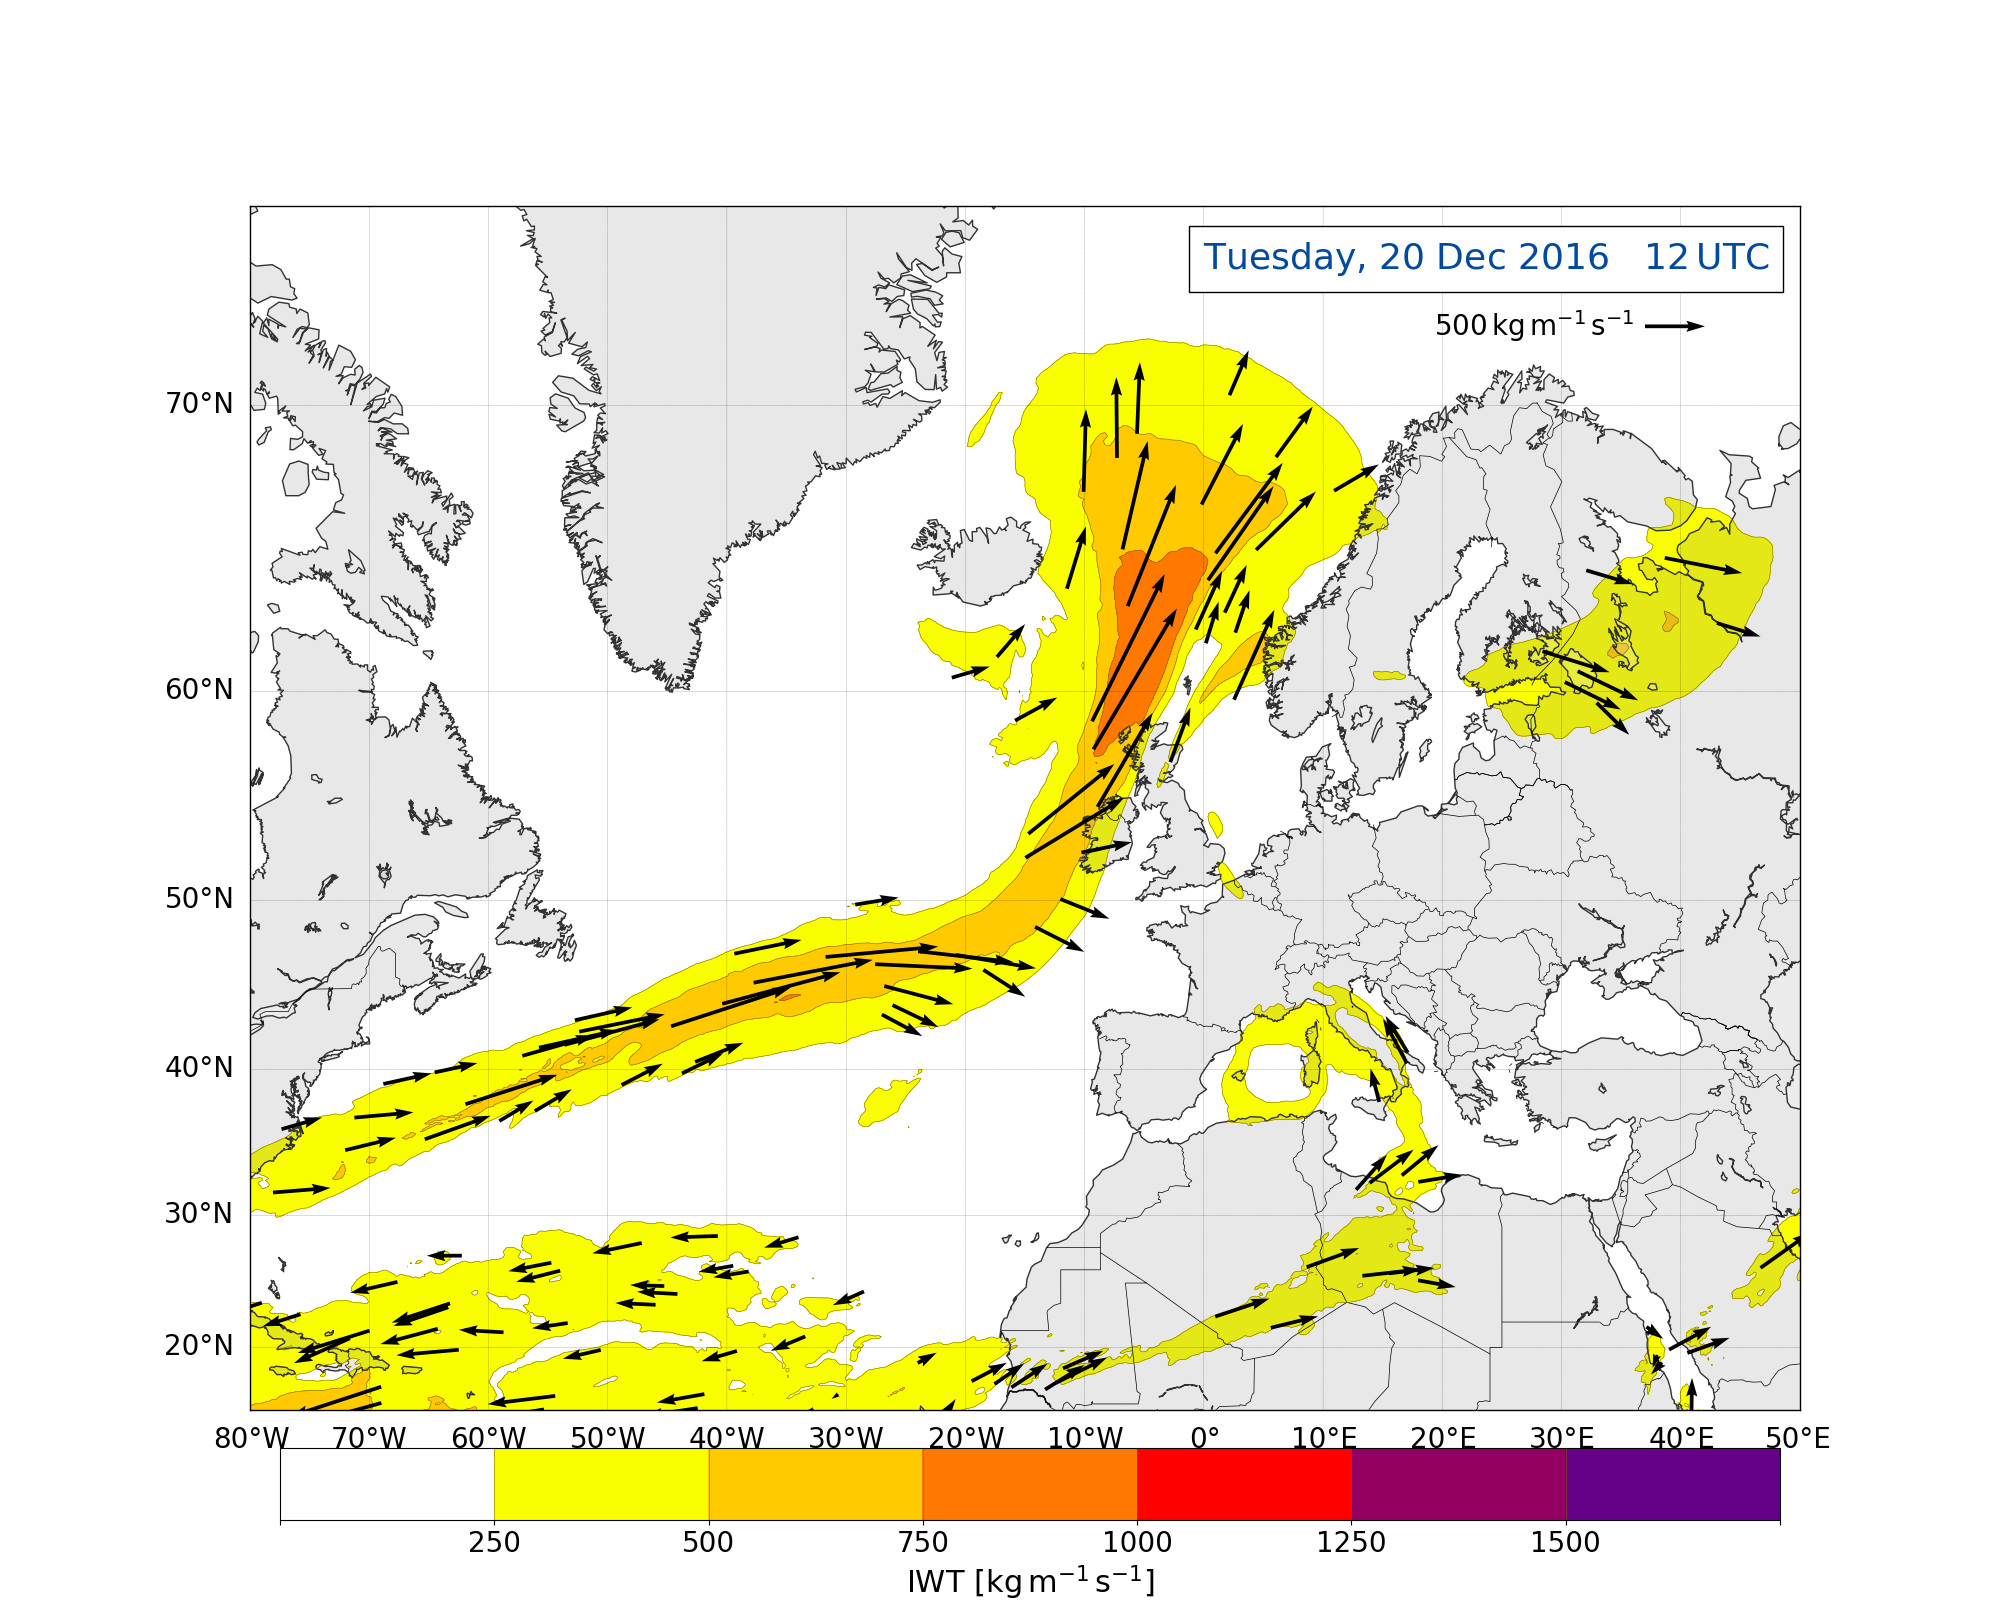
\includegraphics[trim={4.2cm 3.9cm 4.3cm 5.1cm},clip,
		width=\textwidth]{./fig_Atm_Riv/20161220_12}
		\caption{}\label{fig:AR20}
	\end{subfigure}
	%%%%%% 21/12
	\begin{subfigure}[b]{0.49\textwidth}
		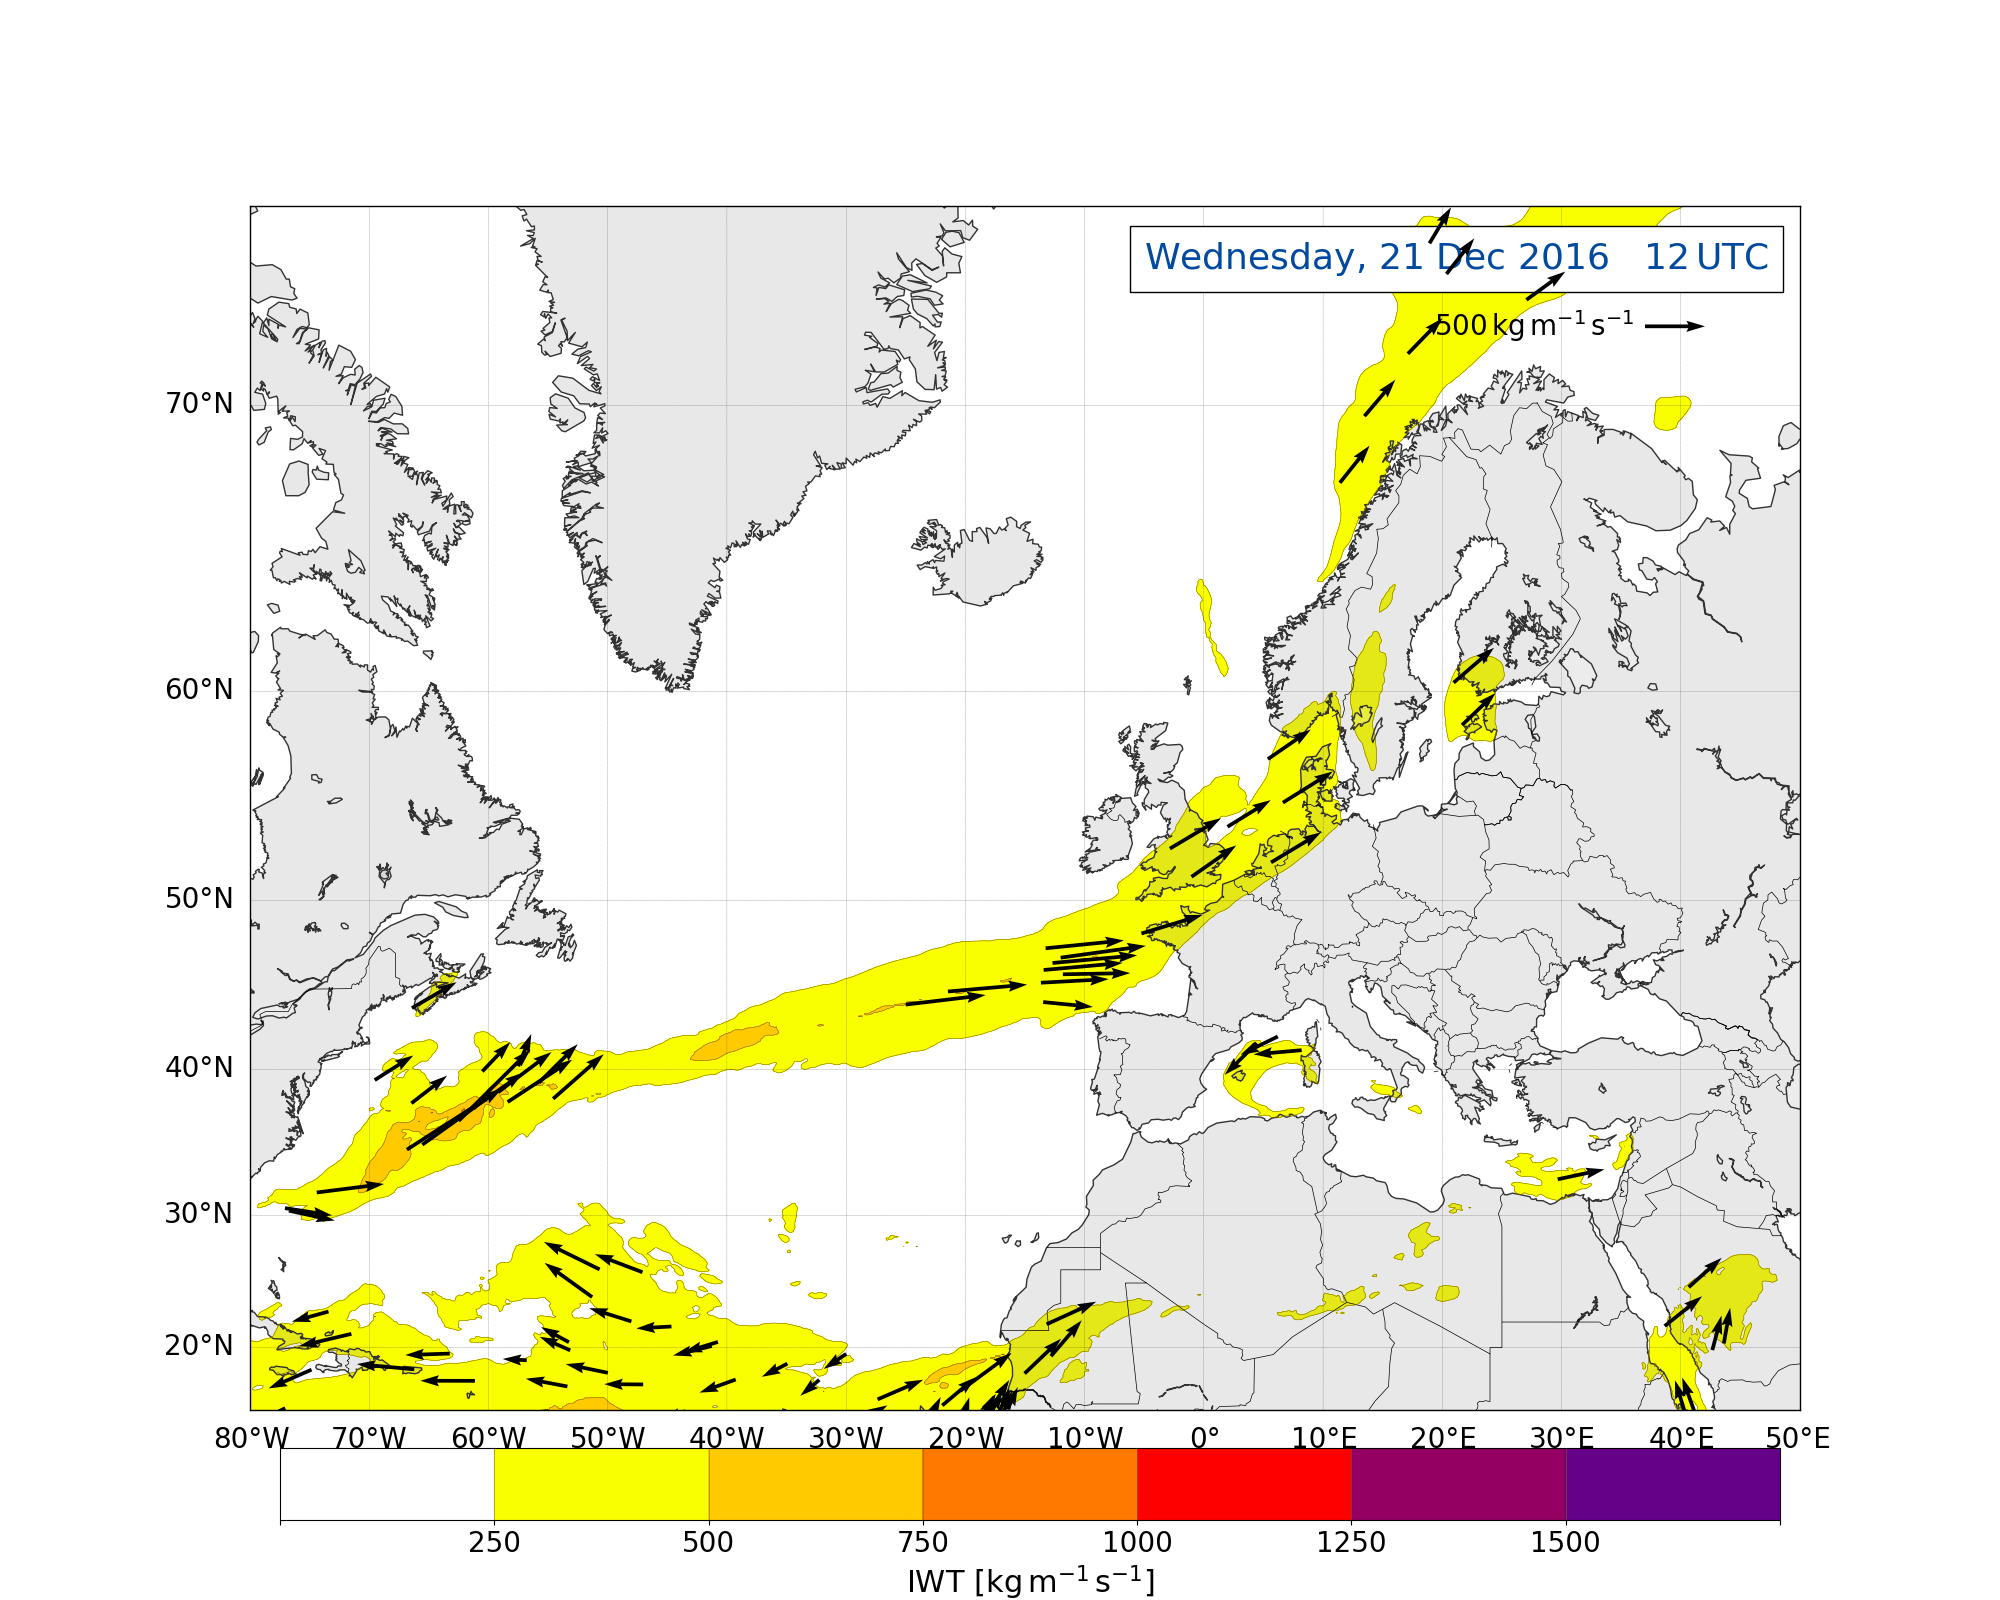
\includegraphics[trim={4.2cm 3.9cm 4.3cm 5.1cm},clip,
		width=\textwidth]{./fig_Atm_Riv/20161221_12}
		\caption{}\label{fig:AR21}
	\end{subfigure}
	%%%%%% label
	\begin{subfigure}[b]{\textwidth}
		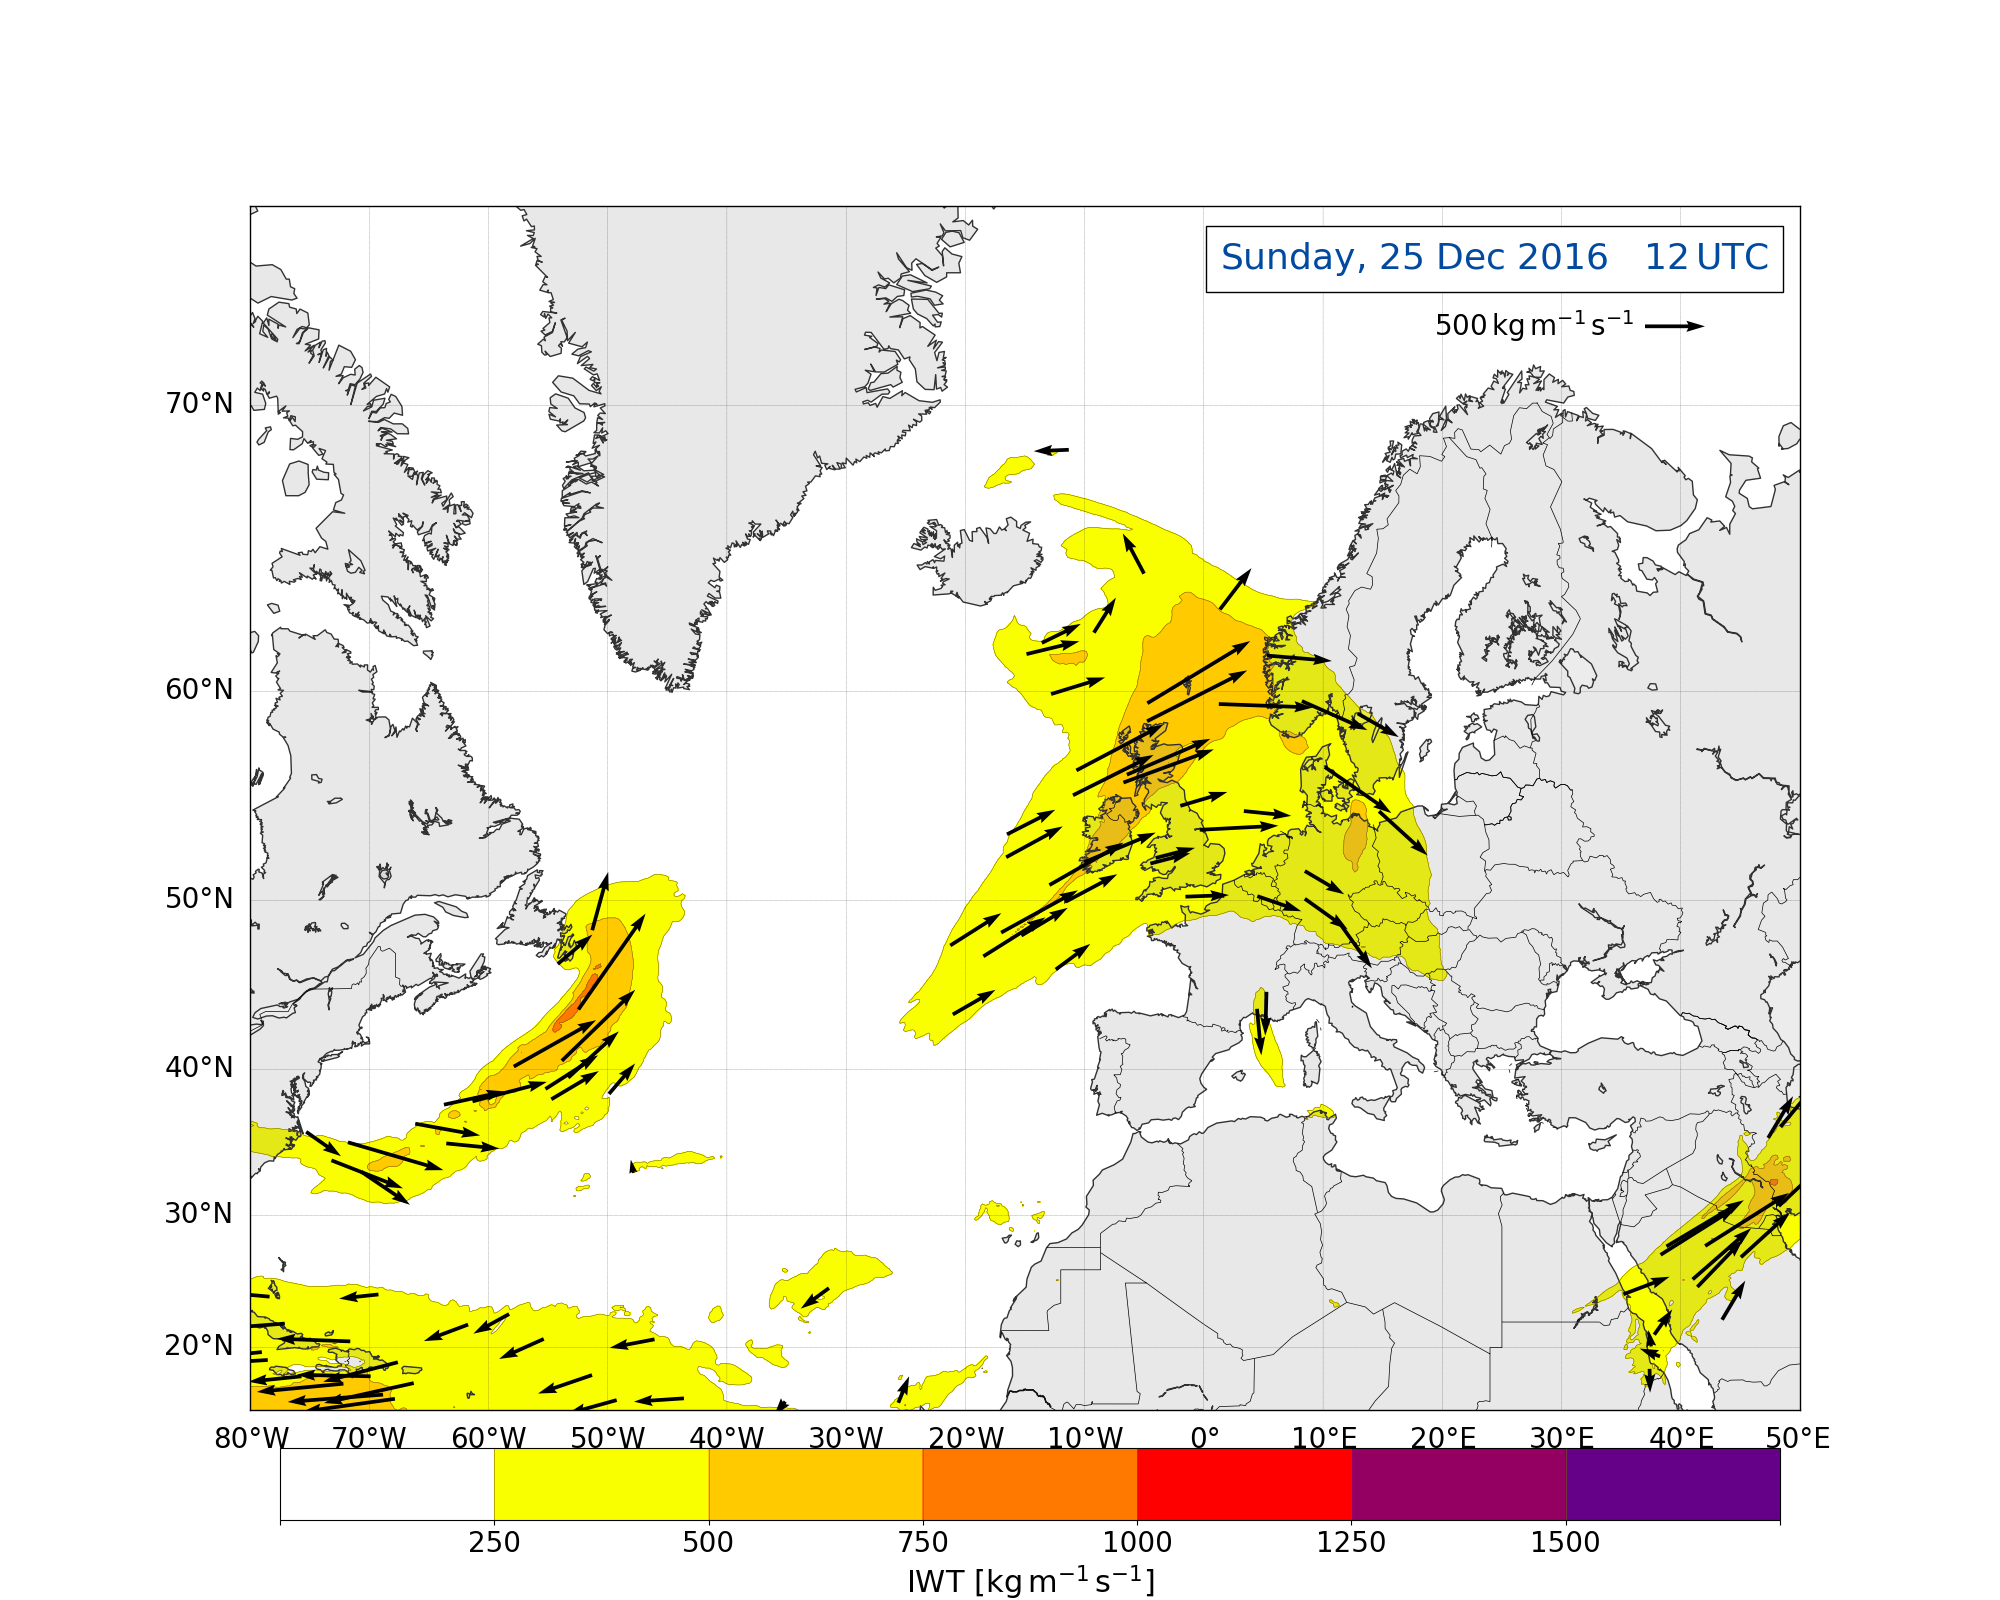
\includegraphics[trim={4.2cm 0cm 4.3cm 36.8cm},clip,
		width=\textwidth]{./fig_Atm_Riv/20161225_12}
	\end{subfigure}
\end{figure}
%
\begin{figure}\ContinuedFloat
	\centering
	%%%%%% 22/12
	\begin{subfigure}[b]{0.49\textwidth}
		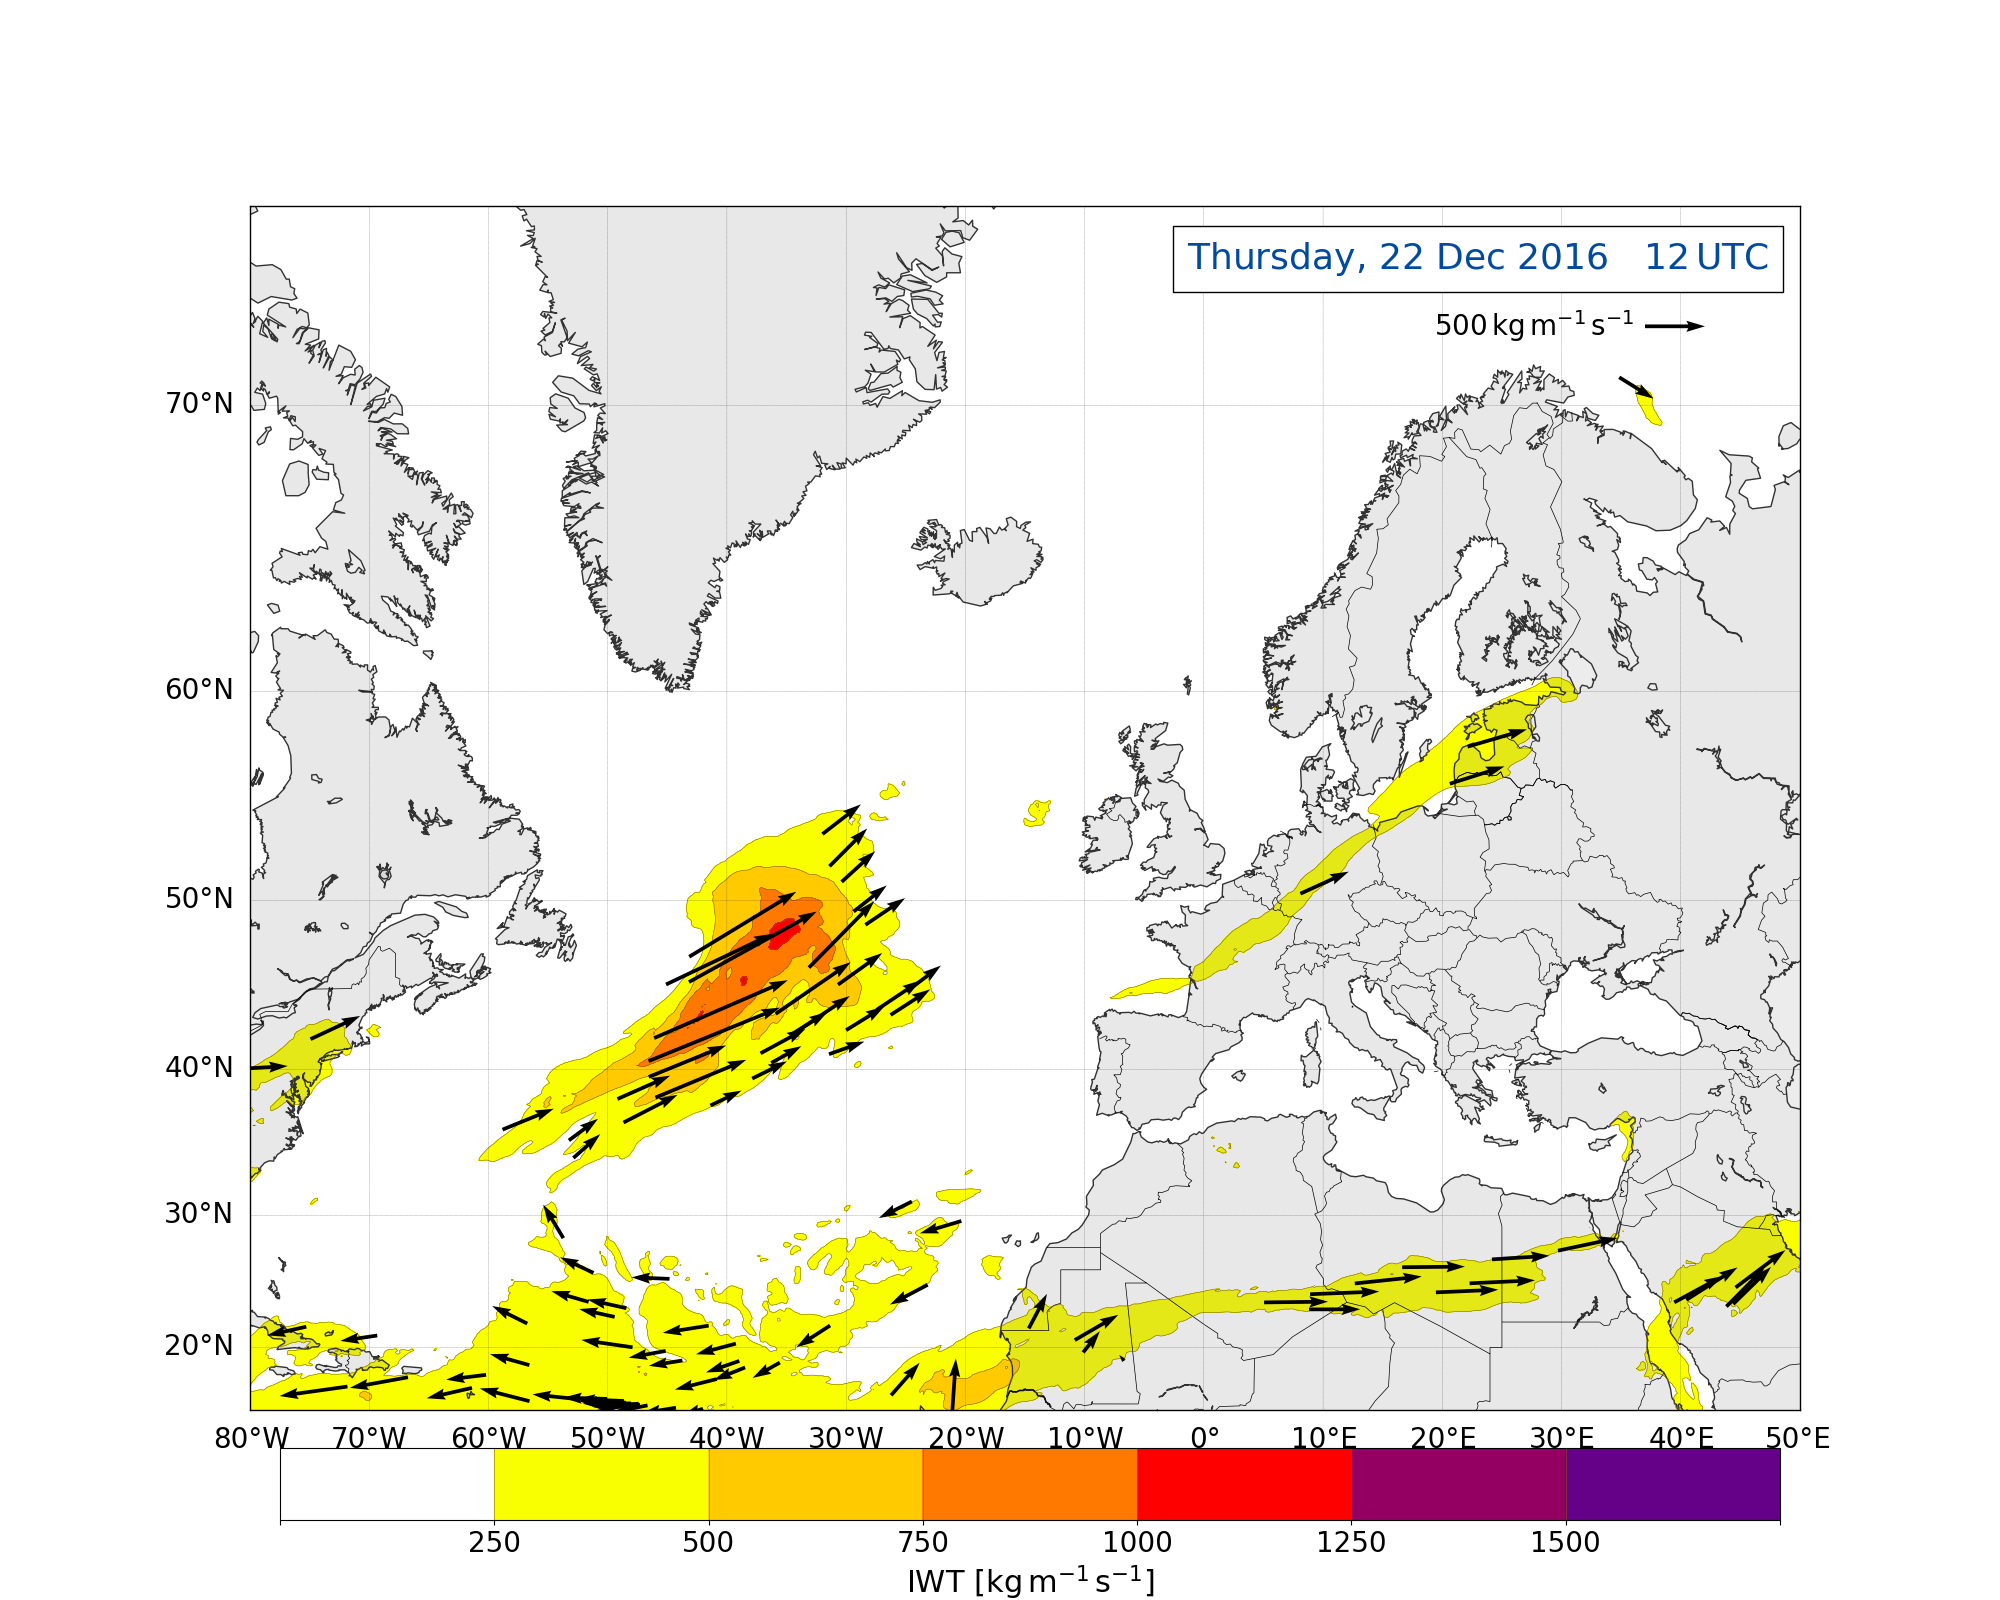
\includegraphics[trim={4.2cm 3.9cm 4.3cm 5.1cm},clip,
		width=\textwidth]{./fig_Atm_Riv/20161222_12}
		\caption{}\label{fig:AR22}
		%\label{fig:sfc2100}
	\end{subfigure}
	%%%%%% 23/12
	\begin{subfigure}[b]{0.49\textwidth}
		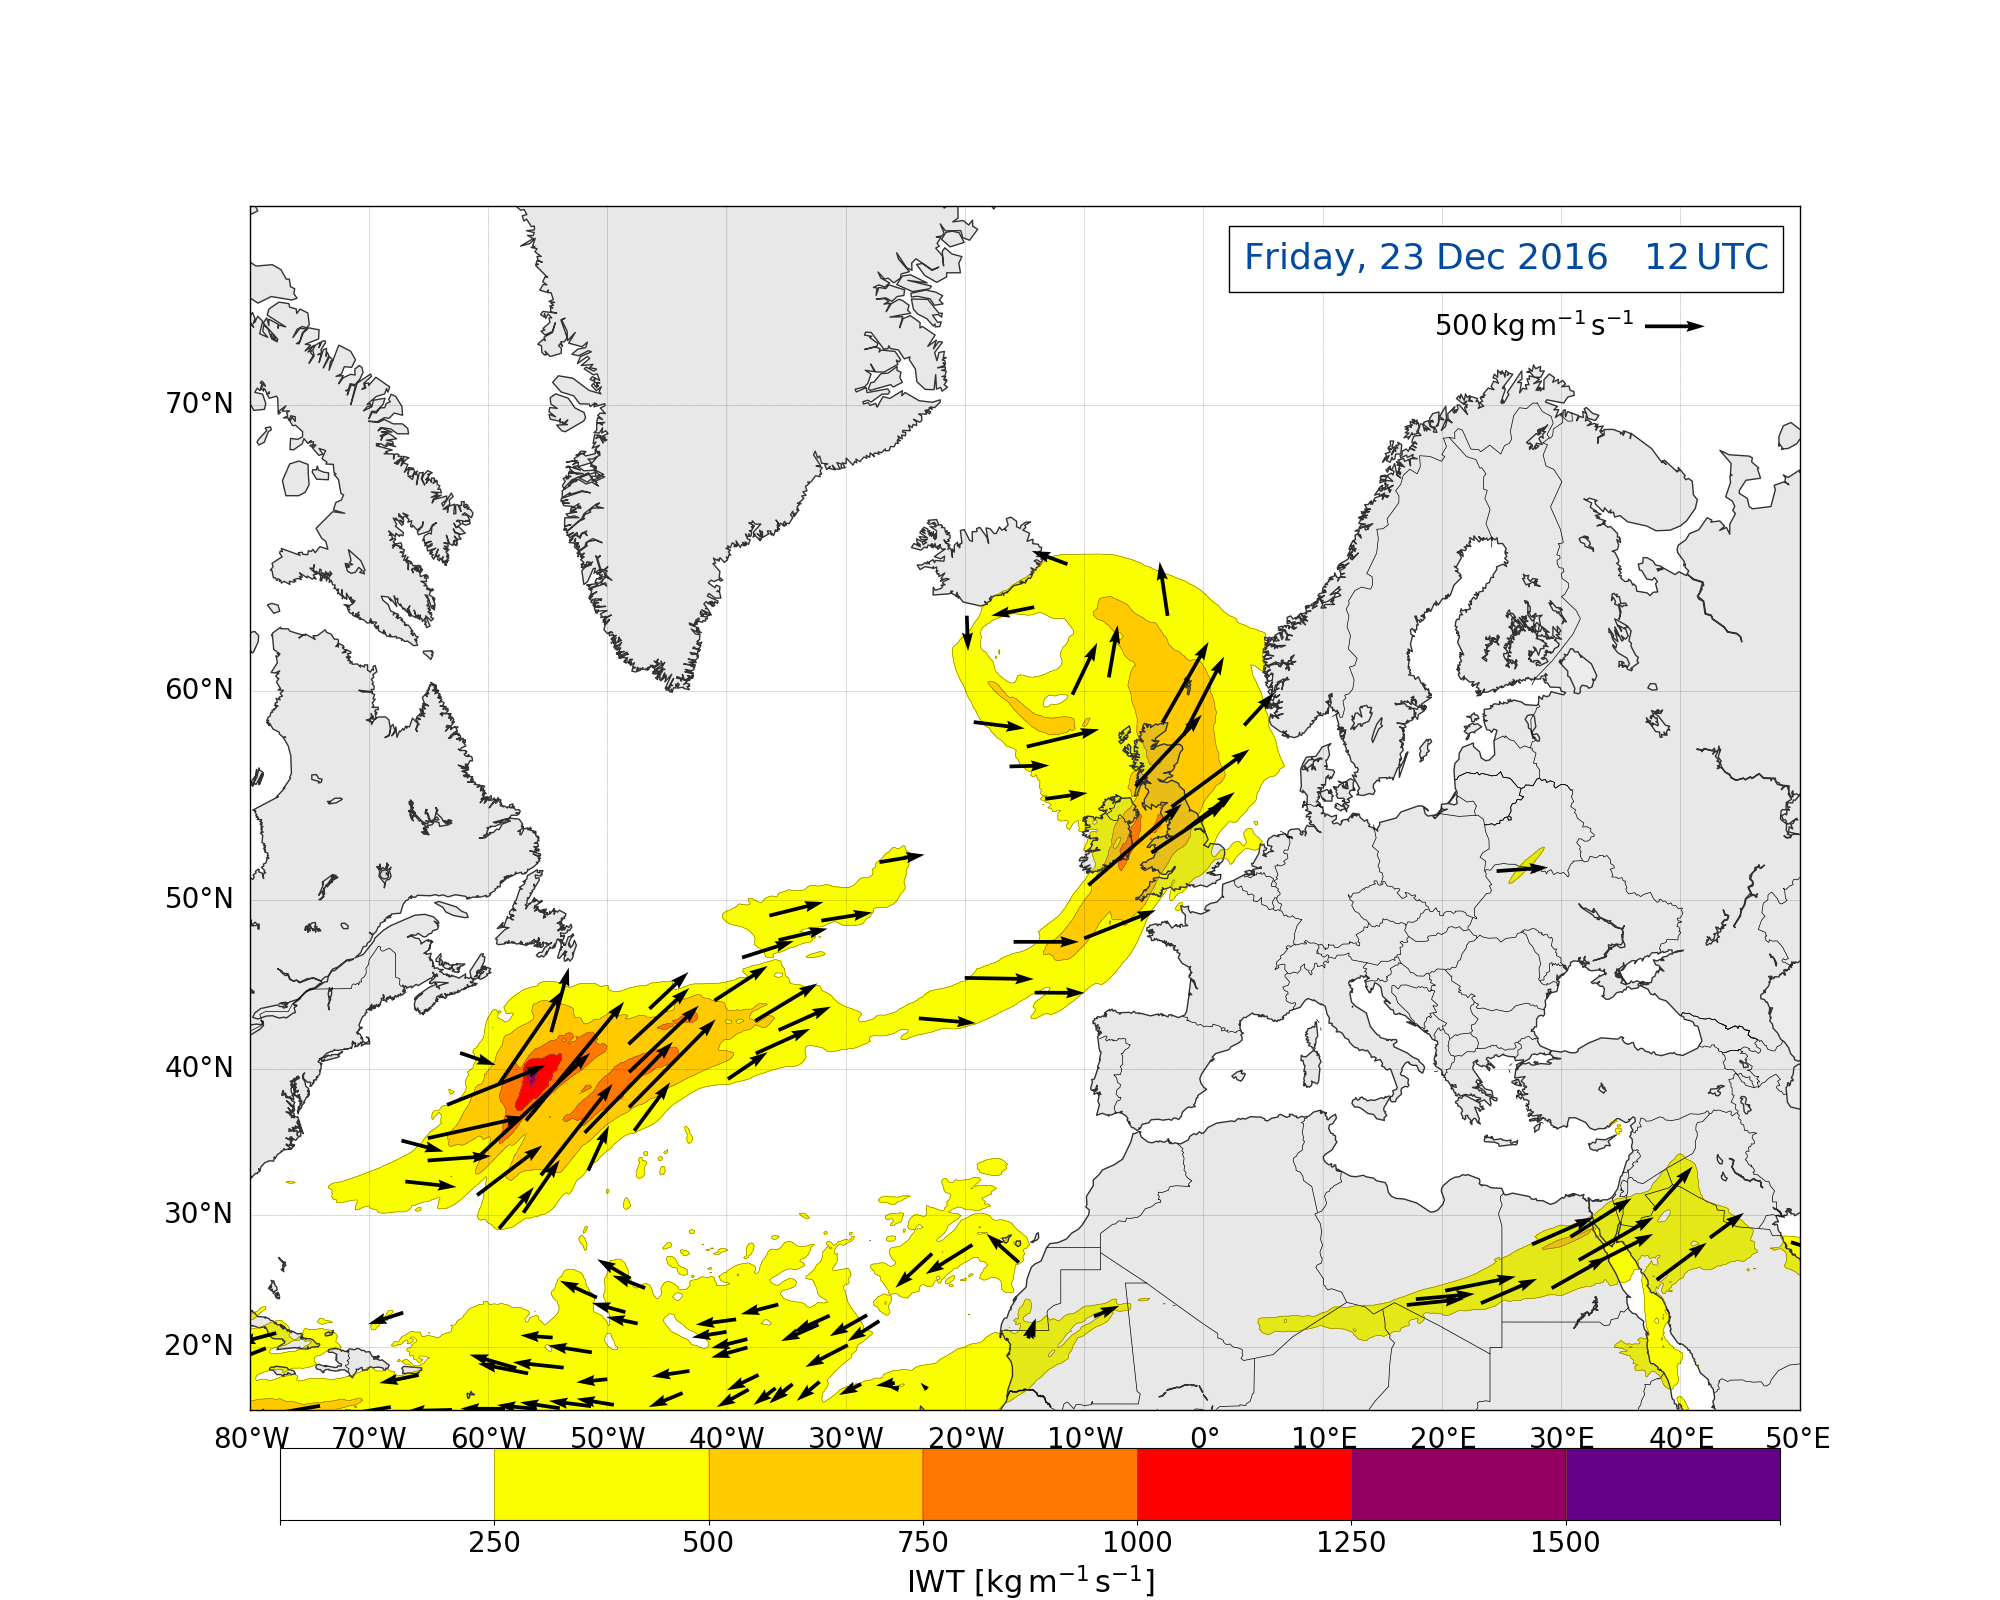
\includegraphics[trim={4.2cm 3.9cm 4.3cm 5.1cm},clip,
		width=\textwidth]{./fig_Atm_Riv/20161223_12}
		\caption{}\label{fig:AR23}
	\end{subfigure}
	%%%%%% 24/12
	\begin{subfigure}[b]{0.49\textwidth}
		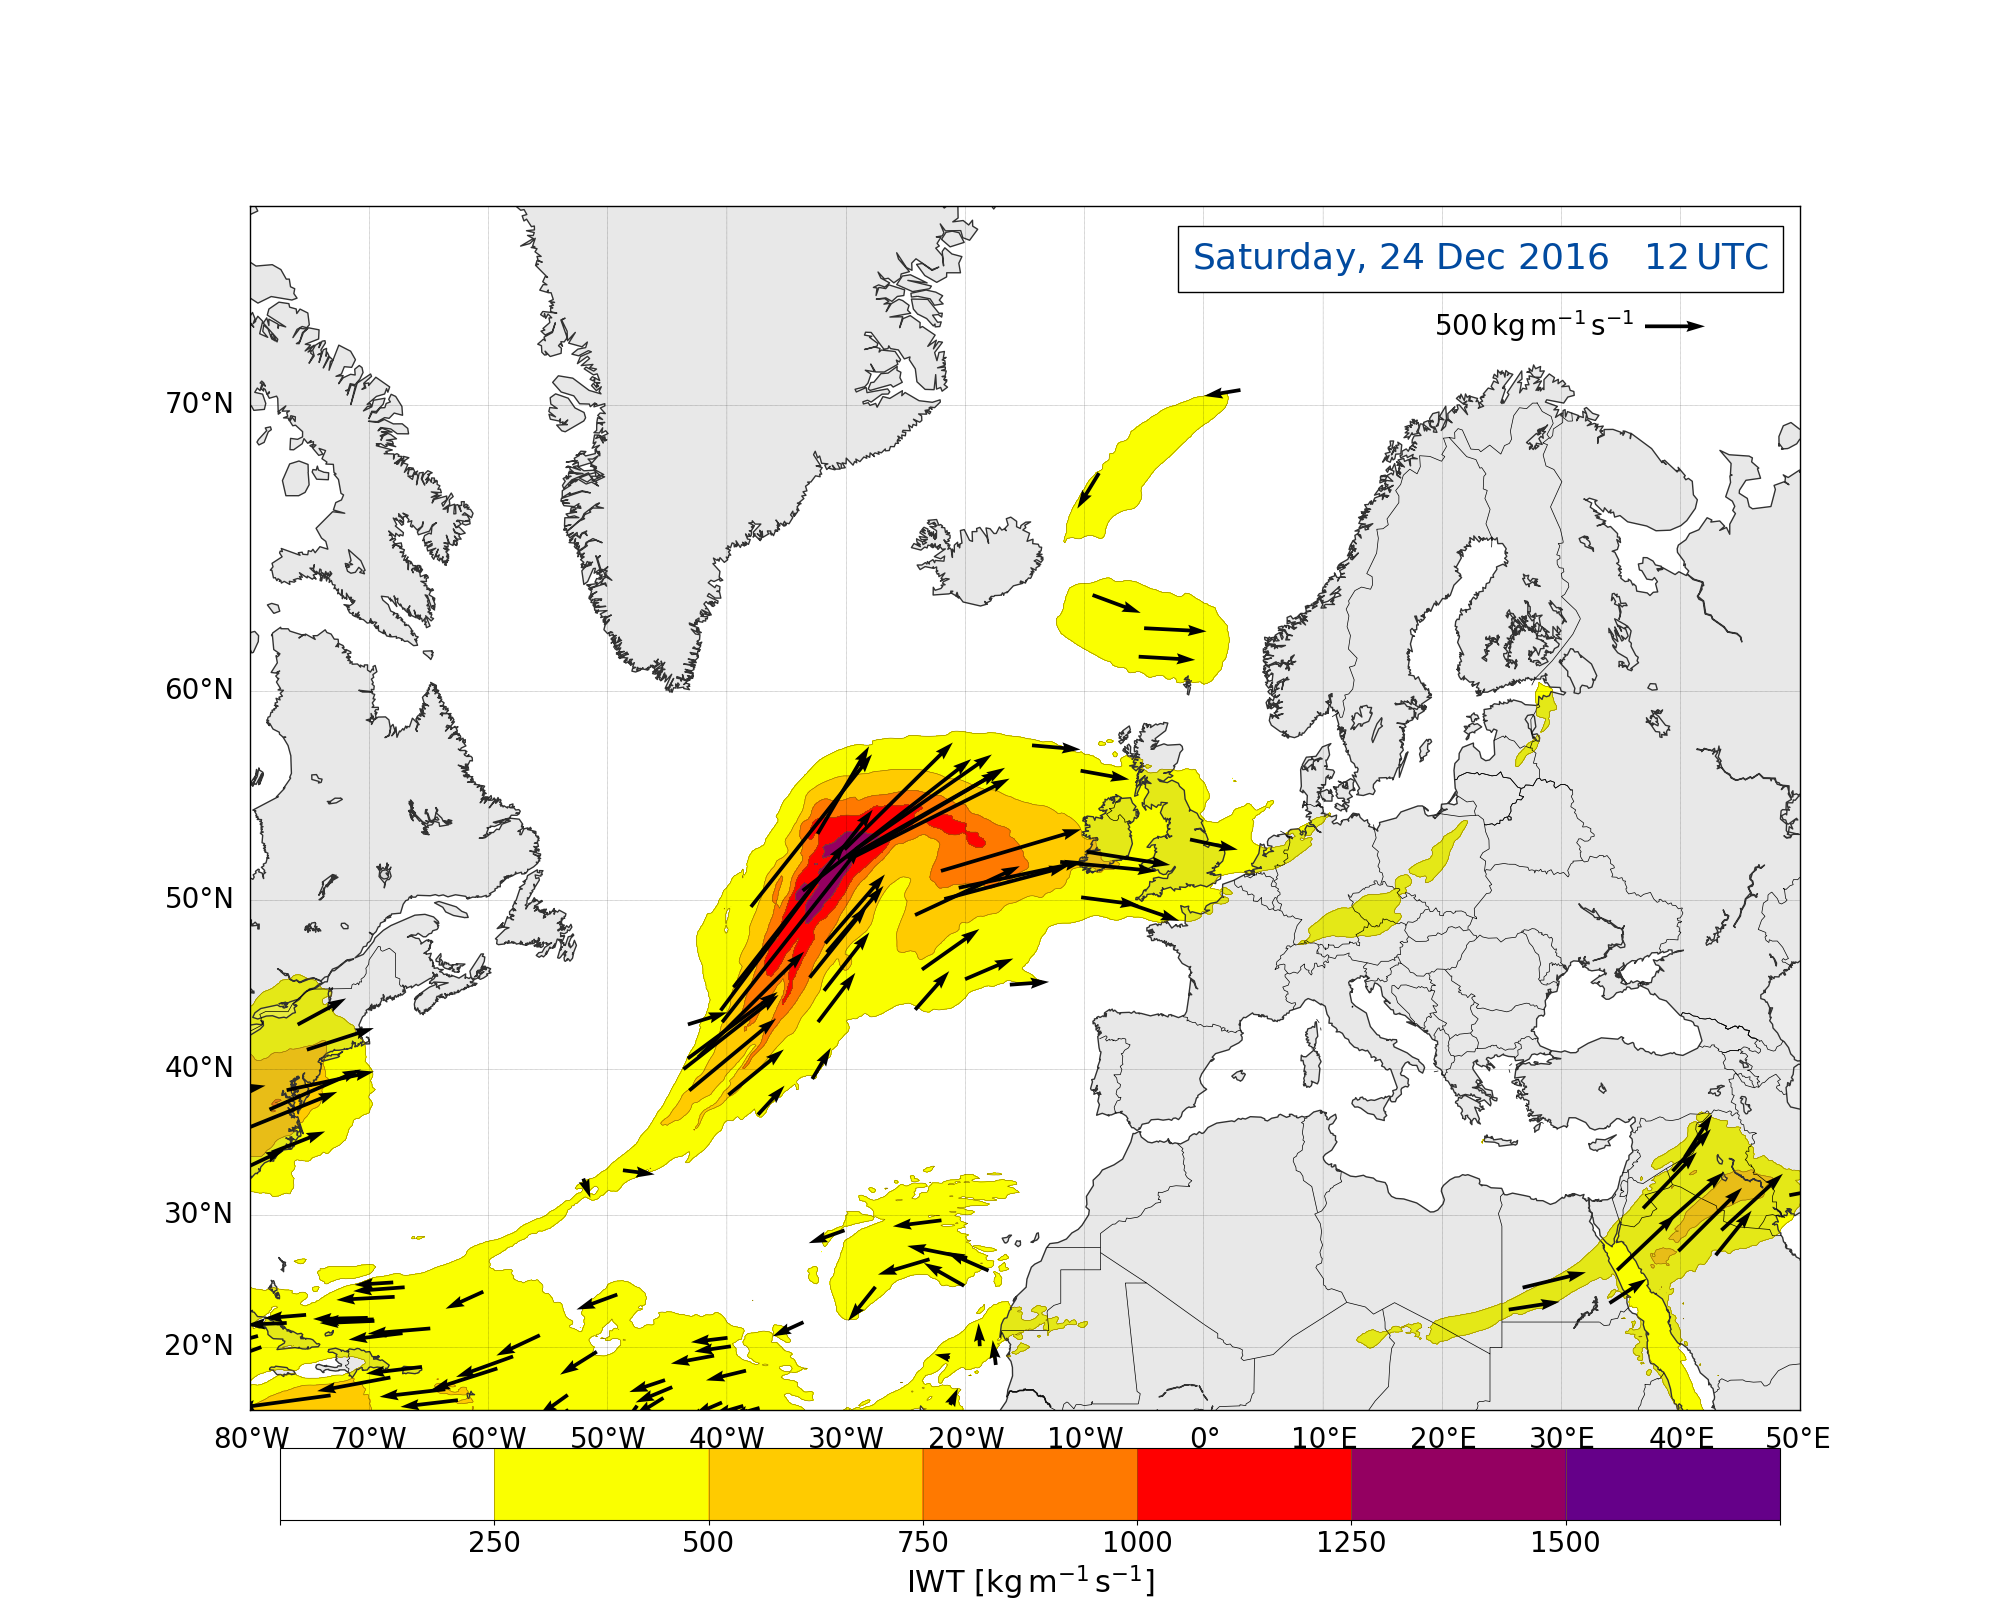
\includegraphics[trim={4.2cm 3.9cm 4.3cm 5.1cm},clip,
		width=\textwidth]{./fig_Atm_Riv/20161224_12}
		\caption{}\label{fig:AR24}
	\end{subfigure}
	%%%%%% 25/12
	\begin{subfigure}[b]{0.49\textwidth}
		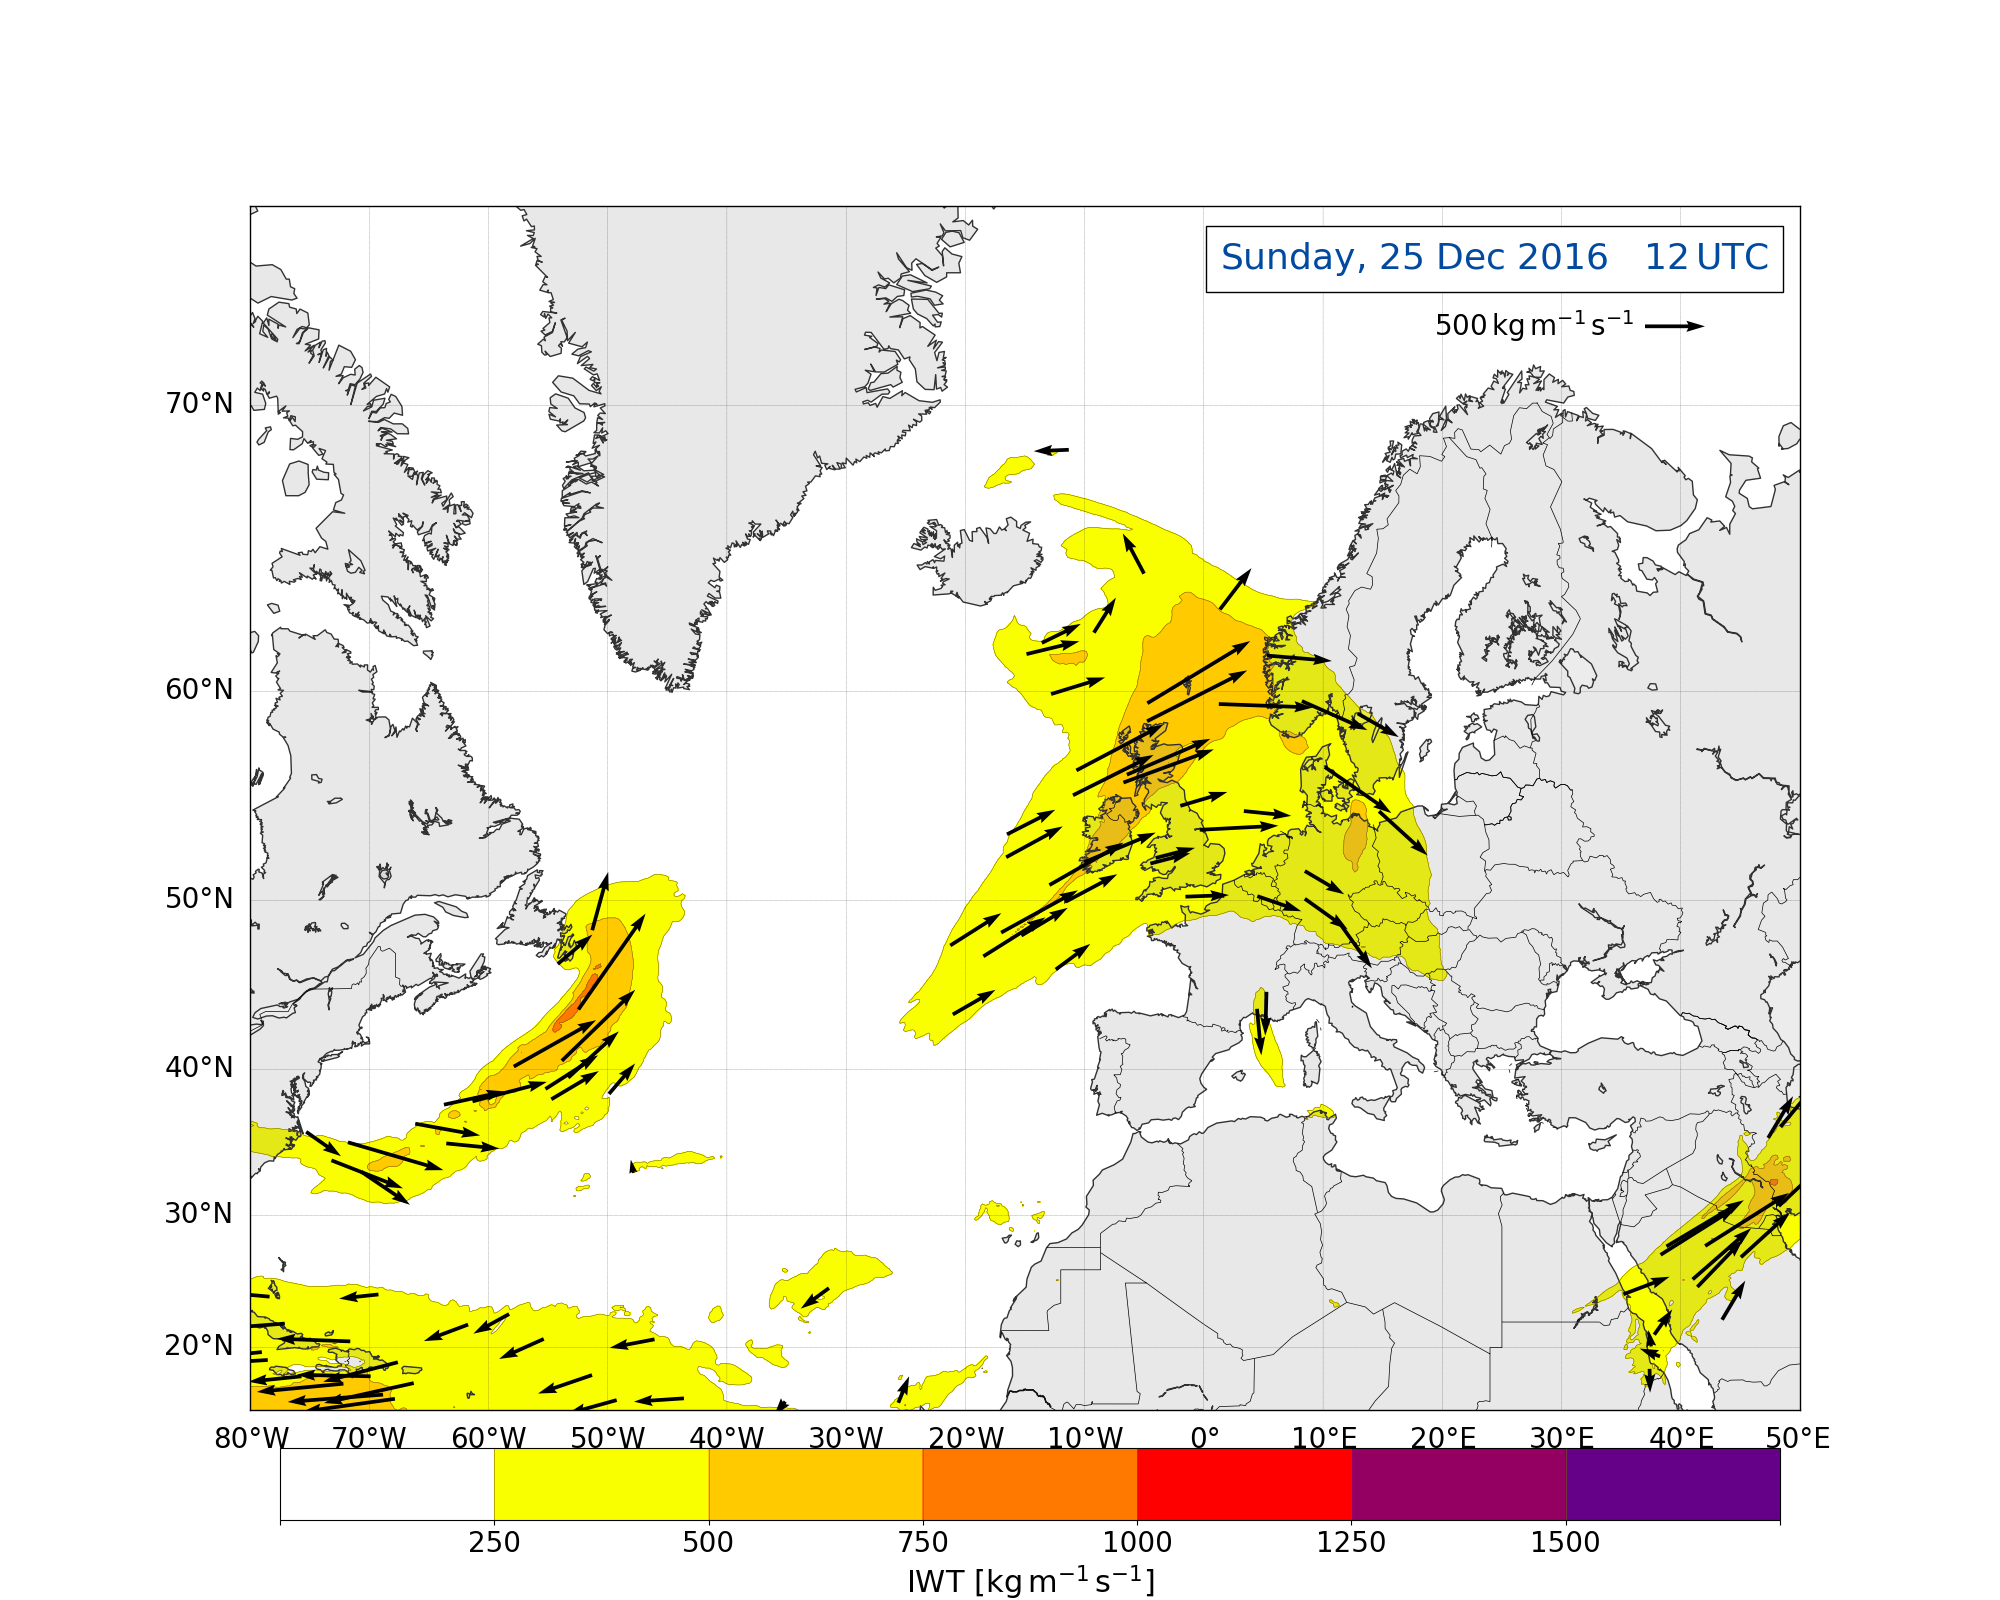
\includegraphics[trim={4.2cm 3.9cm 4.3cm 5.1cm},clip,
		width=\textwidth]{./fig_Atm_Riv/20161225_12}
		\caption{}\label{fig:AR25}
	\end{subfigure}
	%	\centering
	%%%%%% 26/12
	\begin{subfigure}[b]{0.49\textwidth}
		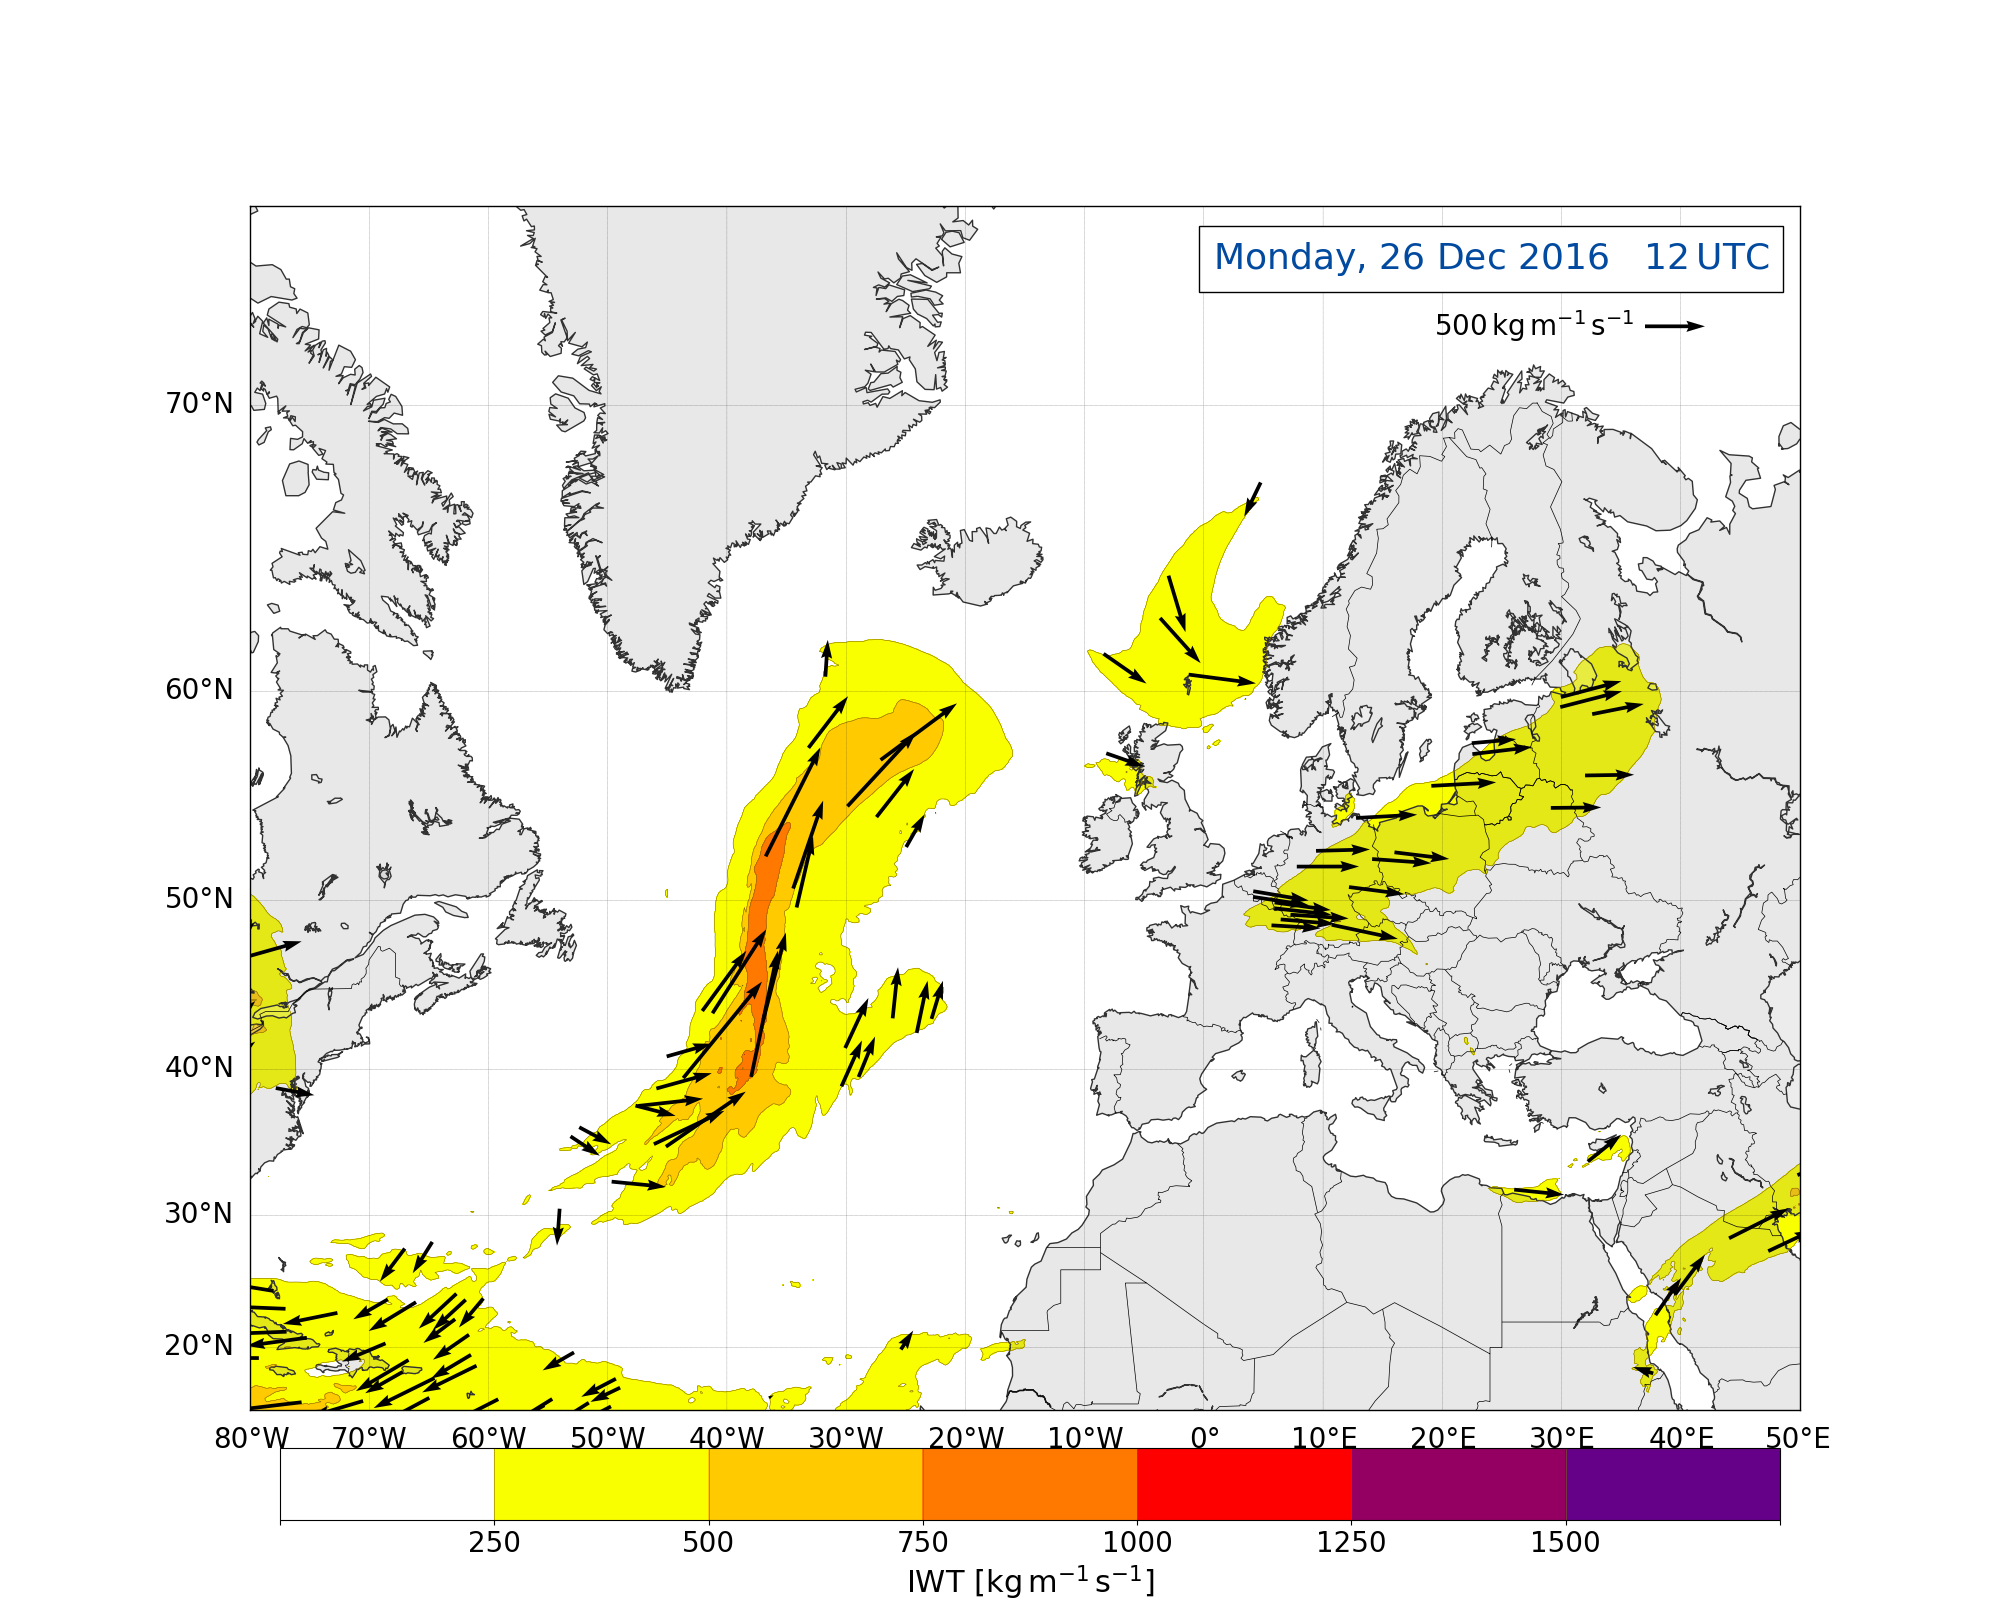
\includegraphics[trim={4.2cm 3.9cm 4.3cm 5.1cm},clip,
		width=\textwidth]{./fig_Atm_Riv/20161226_12}
		\caption{}\label{fig:AR26}
	\end{subfigure}
	%%%%%% 27/12
	\begin{subfigure}[b]{0.49\textwidth}
		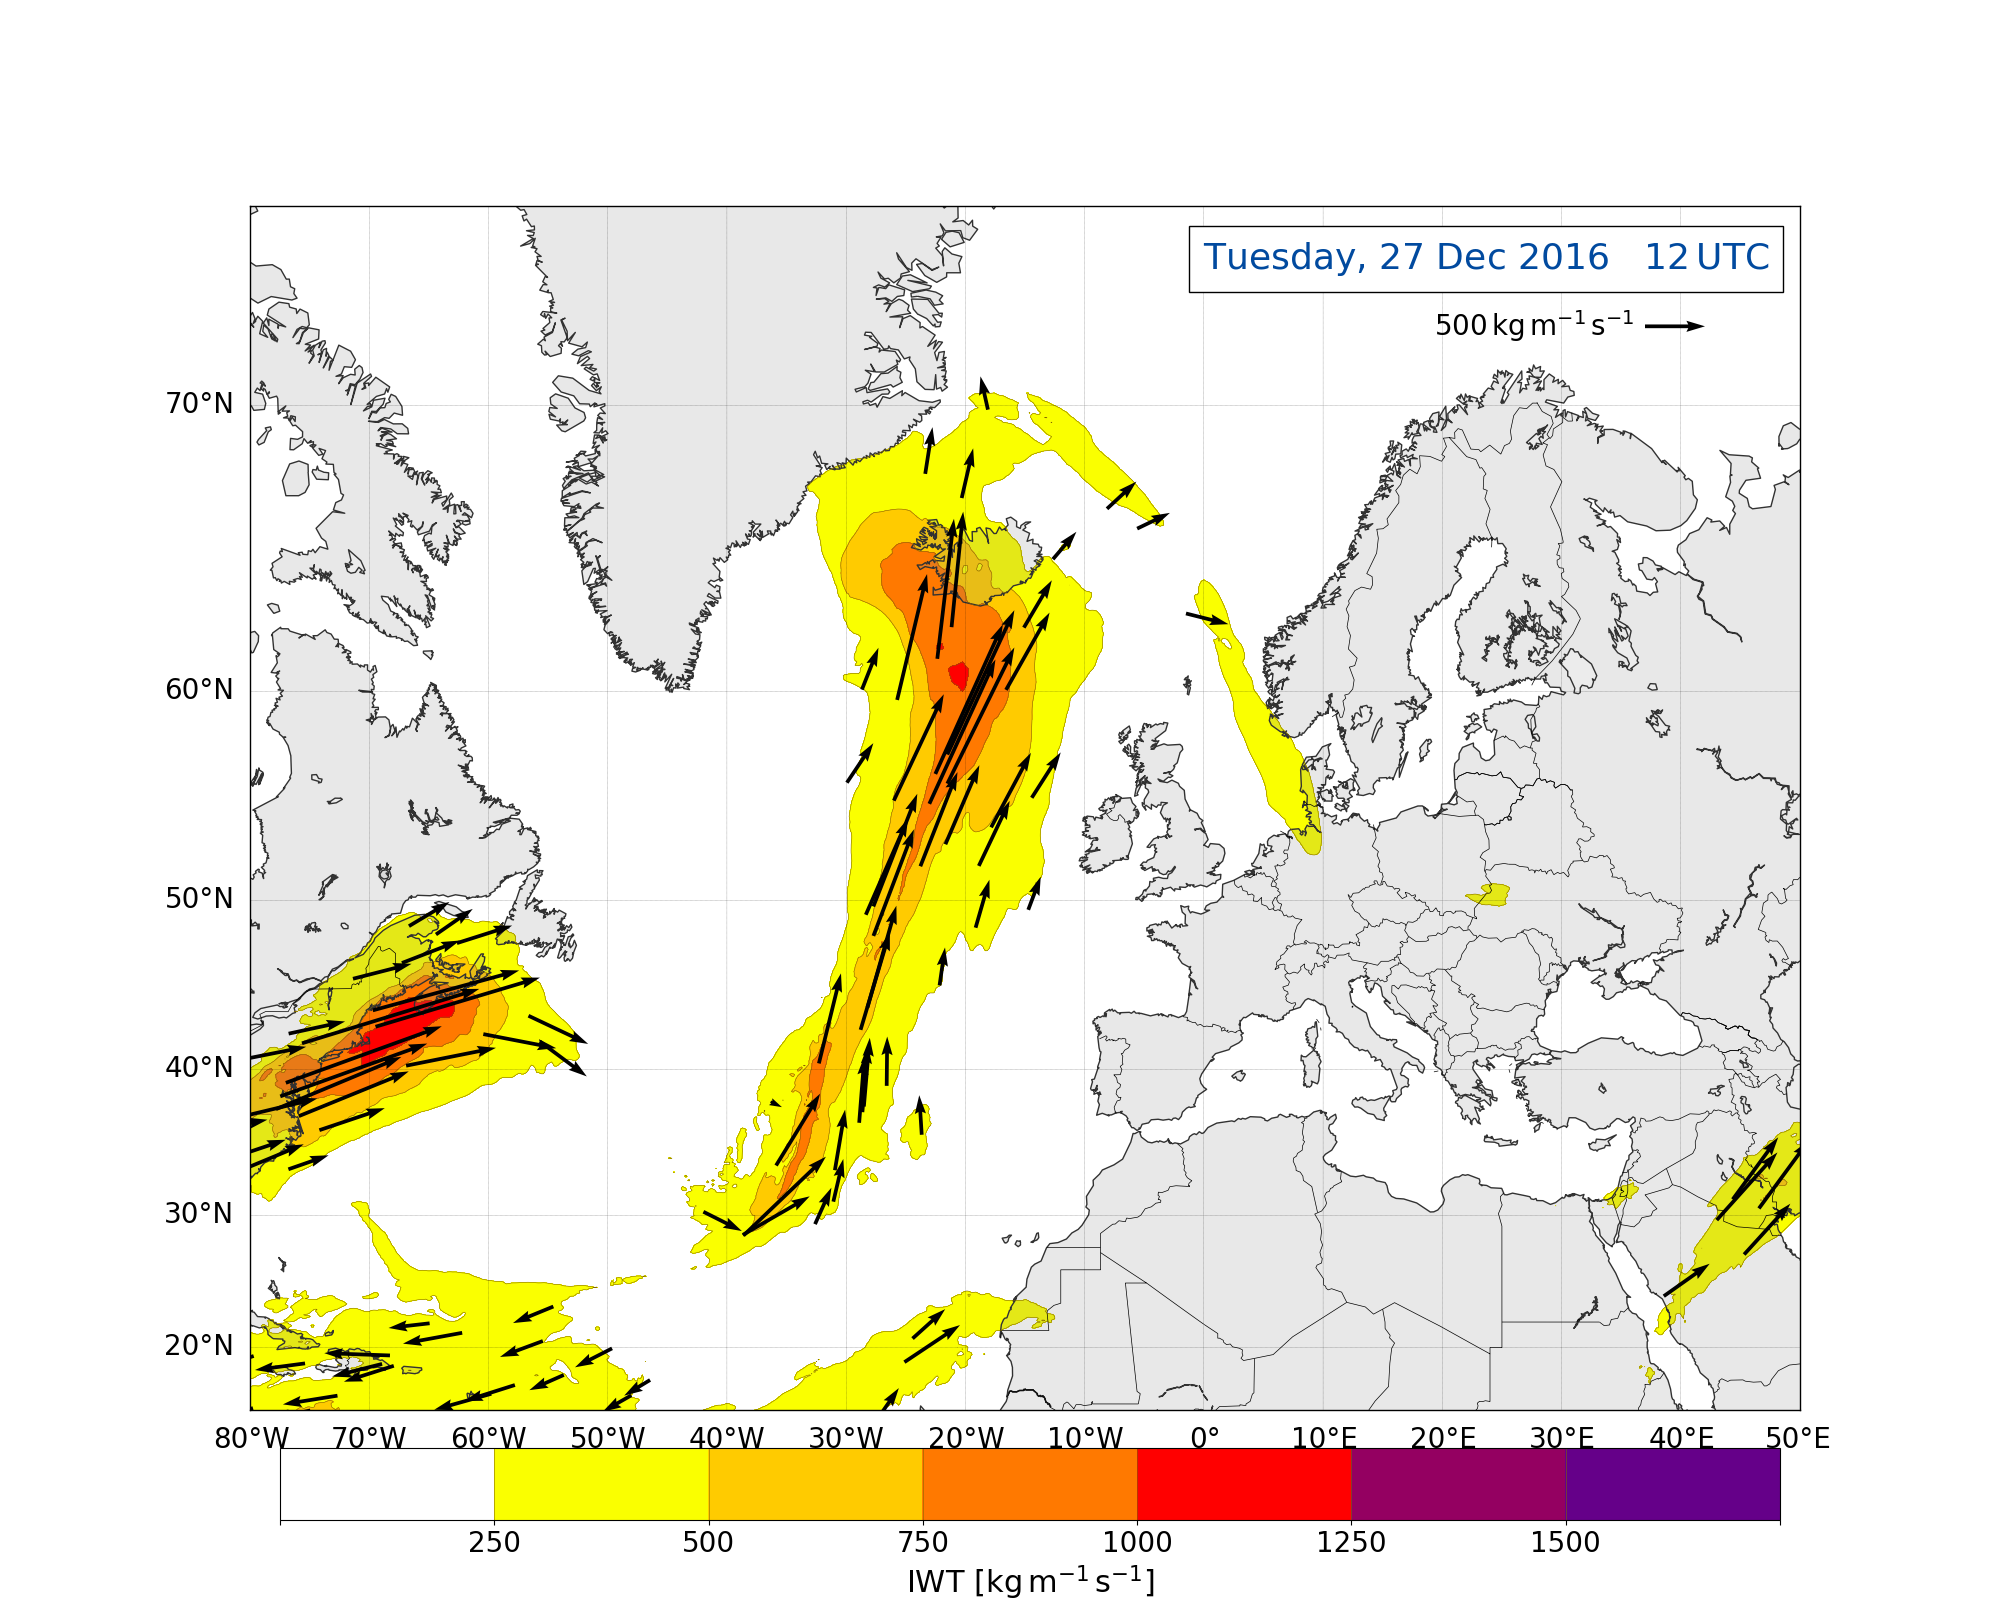
\includegraphics[trim={4.2cm 3.9cm 4.3cm 5.1cm},clip,
		width=\textwidth]{./fig_Atm_Riv/20161227_12}
		\caption{}\label{fig:AR27}
	\end{subfigure}
	%%%%%% label
	\begin{subfigure}[b]{\textwidth}
		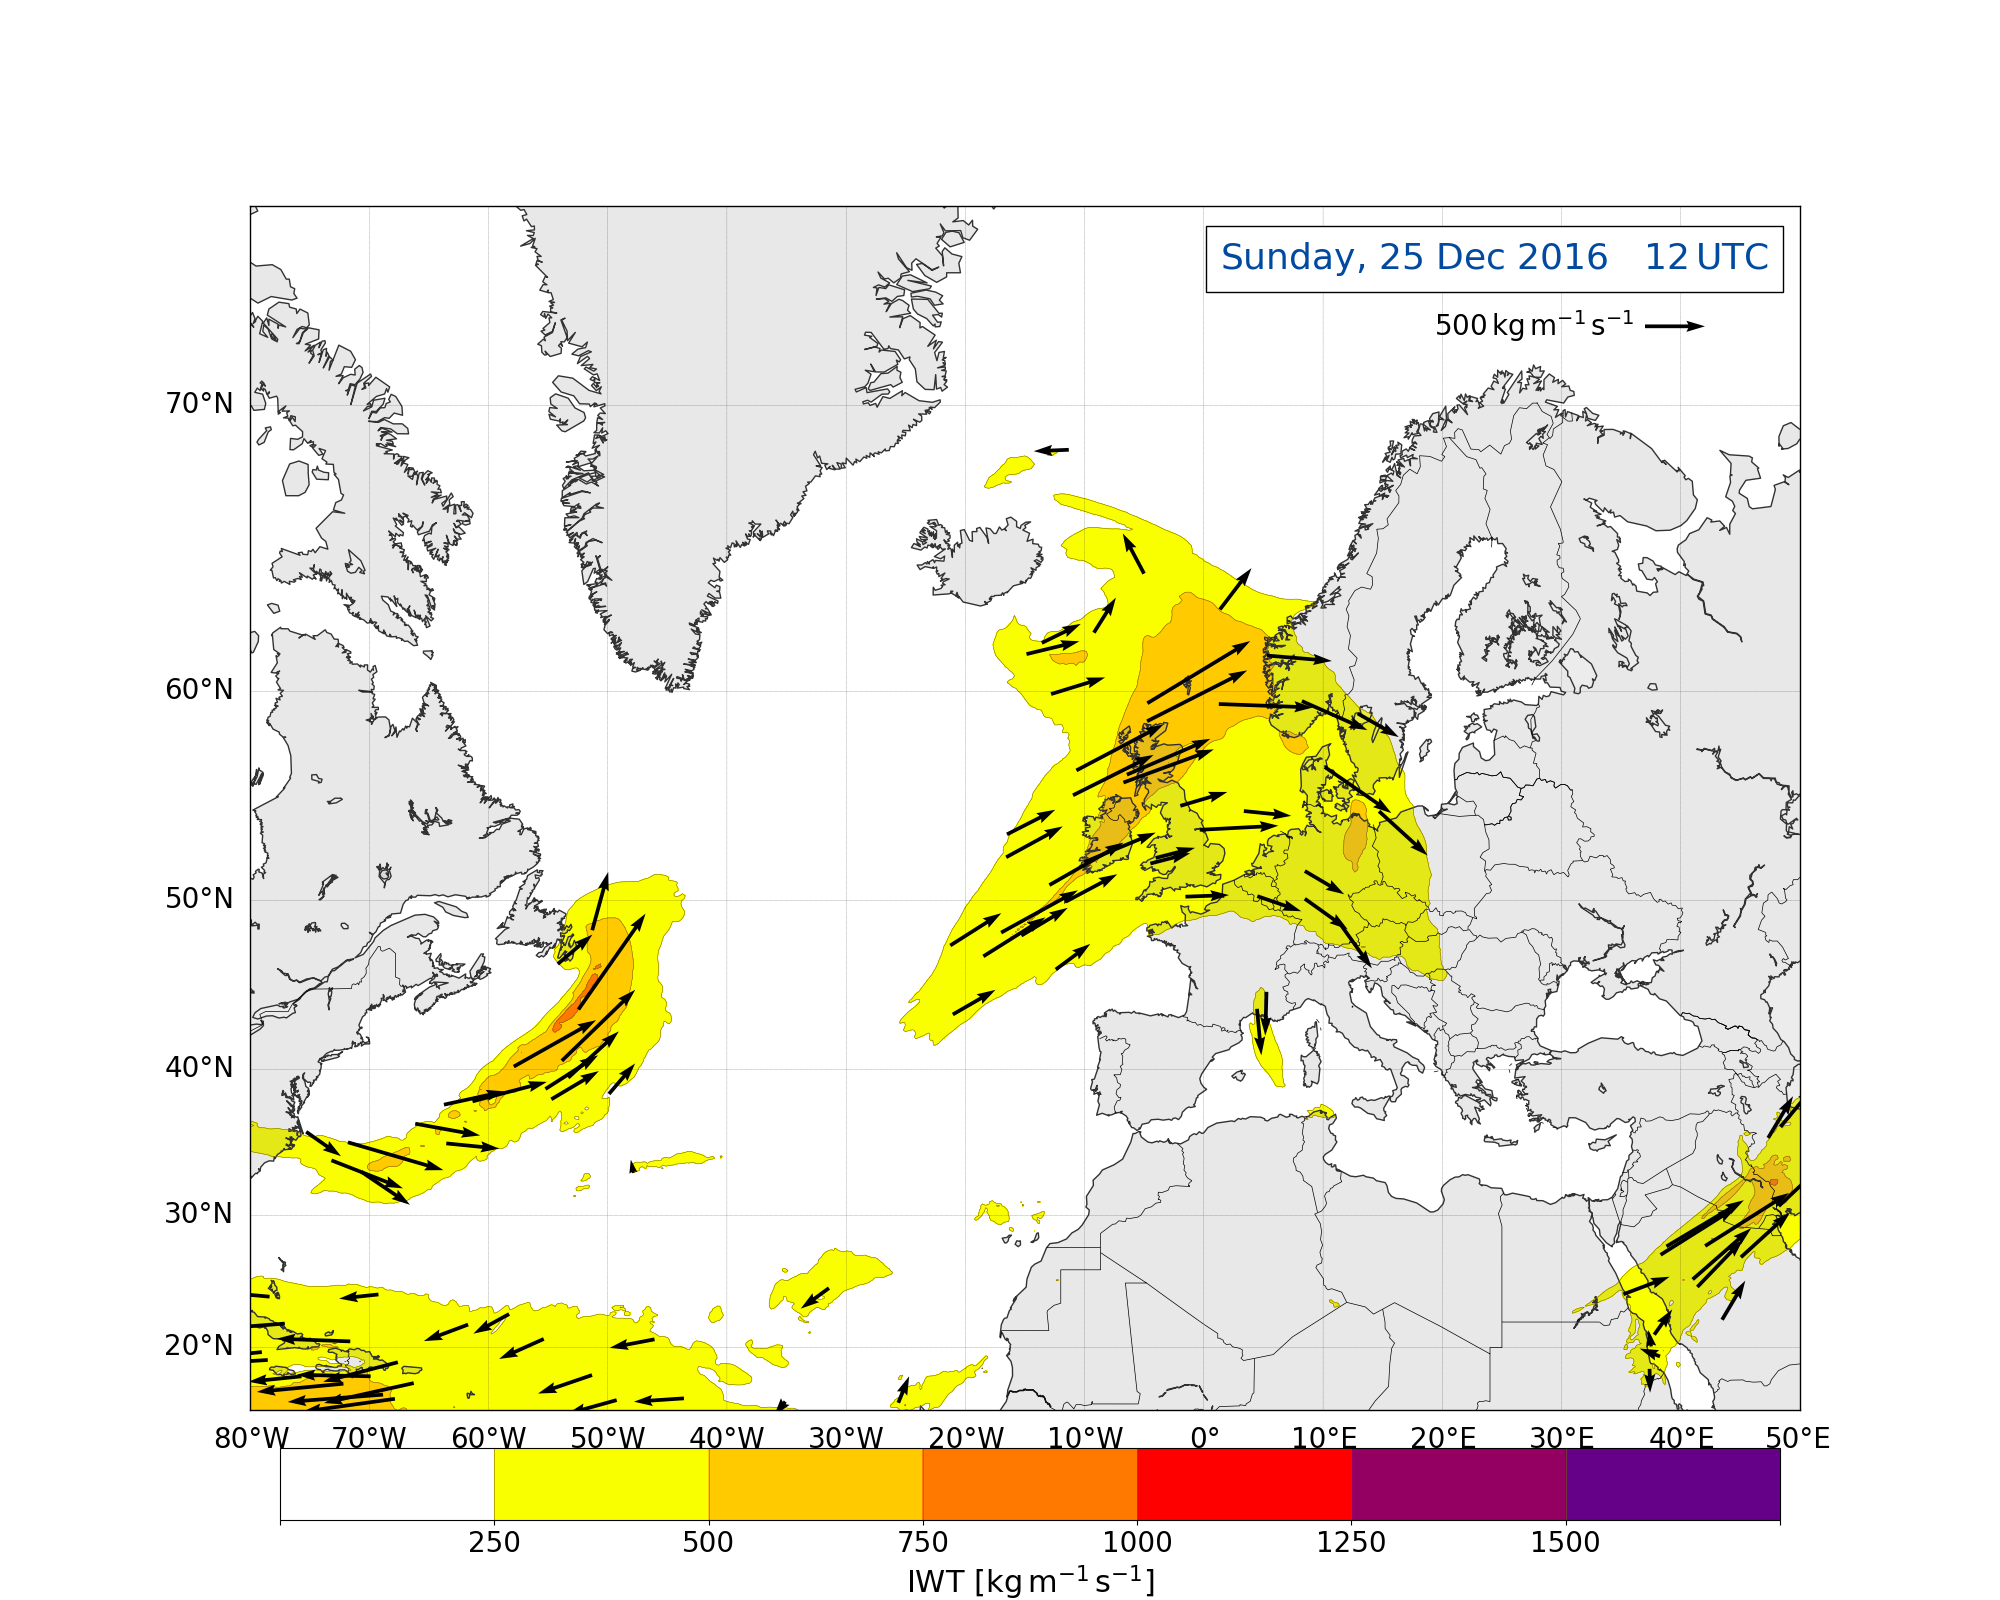
\includegraphics[trim={4.2cm 0cm 4.3cm 36.8cm},clip,
		width=\textwidth]{./fig_Atm_Riv/20161225_12}
	\end{subfigure}
	\caption{Atmospheric river analysis map, data from ECMWF. During \SIrange{20}{27}{\dec}. IVT, shaded according to the colour bar [\SI{}{\IVT}]. Vectors, indicating the direction and magnitude of the IVT. }\label{fig:AtmRiv}
\end{figure}
%%%%%%%%%%%%%%%%%%%%%%%%%%%%%%%%%%%%%%%%%%%%%%%%%%%%%%%%%%%%%%%%%%%%%%%%%%